\documentclass[openany]{book}
\usepackage{lmodern}
\usepackage{amssymb,amsmath}
\usepackage{ifxetex,ifluatex}
\usepackage{fixltx2e} % provides \textsubscript
\ifnum 0\ifxetex 1\fi\ifluatex 1\fi=0 % if pdftex
  \usepackage[T1]{fontenc}
  \usepackage[utf8]{inputenc}
\else % if luatex or xelatex
  \ifxetex
    \usepackage{mathspec}
  \else
    \usepackage{fontspec}
  \fi
  \defaultfontfeatures{Ligatures=TeX,Scale=MatchLowercase}
\fi
% use upquote if available, for straight quotes in verbatim environments
\IfFileExists{upquote.sty}{\usepackage{upquote}}{}
% use microtype if available
\IfFileExists{microtype.sty}{%
\usepackage{microtype}
\UseMicrotypeSet[protrusion]{basicmath} % disable protrusion for tt fonts
}{}
\usepackage[margin=1in]{geometry}
\usepackage{hyperref}
\hypersetup{unicode=true,
            pdftitle={Variable selection in microbiome compositional data analysis: tutorial},
            pdfborder={0 0 0},
            breaklinks=true}
\urlstyle{same}  % don't use monospace font for urls
\usepackage{natbib}
\bibliographystyle{apalike}
\usepackage{color}
\usepackage{fancyvrb}
\newcommand{\VerbBar}{|}
\newcommand{\VERB}{\Verb[commandchars=\\\{\}]}
\DefineVerbatimEnvironment{Highlighting}{Verbatim}{commandchars=\\\{\}}
% Add ',fontsize=\small' for more characters per line
\usepackage{framed}
\definecolor{shadecolor}{RGB}{248,248,248}
\newenvironment{Shaded}{\begin{snugshade}}{\end{snugshade}}
\newcommand{\KeywordTok}[1]{\textcolor[rgb]{0.13,0.29,0.53}{\textbf{#1}}}
\newcommand{\DataTypeTok}[1]{\textcolor[rgb]{0.13,0.29,0.53}{#1}}
\newcommand{\DecValTok}[1]{\textcolor[rgb]{0.00,0.00,0.81}{#1}}
\newcommand{\BaseNTok}[1]{\textcolor[rgb]{0.00,0.00,0.81}{#1}}
\newcommand{\FloatTok}[1]{\textcolor[rgb]{0.00,0.00,0.81}{#1}}
\newcommand{\ConstantTok}[1]{\textcolor[rgb]{0.00,0.00,0.00}{#1}}
\newcommand{\CharTok}[1]{\textcolor[rgb]{0.31,0.60,0.02}{#1}}
\newcommand{\SpecialCharTok}[1]{\textcolor[rgb]{0.00,0.00,0.00}{#1}}
\newcommand{\StringTok}[1]{\textcolor[rgb]{0.31,0.60,0.02}{#1}}
\newcommand{\VerbatimStringTok}[1]{\textcolor[rgb]{0.31,0.60,0.02}{#1}}
\newcommand{\SpecialStringTok}[1]{\textcolor[rgb]{0.31,0.60,0.02}{#1}}
\newcommand{\ImportTok}[1]{#1}
\newcommand{\CommentTok}[1]{\textcolor[rgb]{0.56,0.35,0.01}{\textit{#1}}}
\newcommand{\DocumentationTok}[1]{\textcolor[rgb]{0.56,0.35,0.01}{\textbf{\textit{#1}}}}
\newcommand{\AnnotationTok}[1]{\textcolor[rgb]{0.56,0.35,0.01}{\textbf{\textit{#1}}}}
\newcommand{\CommentVarTok}[1]{\textcolor[rgb]{0.56,0.35,0.01}{\textbf{\textit{#1}}}}
\newcommand{\OtherTok}[1]{\textcolor[rgb]{0.56,0.35,0.01}{#1}}
\newcommand{\FunctionTok}[1]{\textcolor[rgb]{0.00,0.00,0.00}{#1}}
\newcommand{\VariableTok}[1]{\textcolor[rgb]{0.00,0.00,0.00}{#1}}
\newcommand{\ControlFlowTok}[1]{\textcolor[rgb]{0.13,0.29,0.53}{\textbf{#1}}}
\newcommand{\OperatorTok}[1]{\textcolor[rgb]{0.81,0.36,0.00}{\textbf{#1}}}
\newcommand{\BuiltInTok}[1]{#1}
\newcommand{\ExtensionTok}[1]{#1}
\newcommand{\PreprocessorTok}[1]{\textcolor[rgb]{0.56,0.35,0.01}{\textit{#1}}}
\newcommand{\AttributeTok}[1]{\textcolor[rgb]{0.77,0.63,0.00}{#1}}
\newcommand{\RegionMarkerTok}[1]{#1}
\newcommand{\InformationTok}[1]{\textcolor[rgb]{0.56,0.35,0.01}{\textbf{\textit{#1}}}}
\newcommand{\WarningTok}[1]{\textcolor[rgb]{0.56,0.35,0.01}{\textbf{\textit{#1}}}}
\newcommand{\AlertTok}[1]{\textcolor[rgb]{0.94,0.16,0.16}{#1}}
\newcommand{\ErrorTok}[1]{\textcolor[rgb]{0.64,0.00,0.00}{\textbf{#1}}}
\newcommand{\NormalTok}[1]{#1}
\usepackage{longtable,booktabs}
\usepackage{graphicx,grffile}
\makeatletter
\def\maxwidth{\ifdim\Gin@nat@width>\linewidth\linewidth\else\Gin@nat@width\fi}
\def\maxheight{\ifdim\Gin@nat@height>\textheight\textheight\else\Gin@nat@height\fi}
\makeatother
% Scale images if necessary, so that they will not overflow the page
% margins by default, and it is still possible to overwrite the defaults
% using explicit options in \includegraphics[width, height, ...]{}
\setkeys{Gin}{width=\maxwidth,height=\maxheight,keepaspectratio}
\IfFileExists{parskip.sty}{%
\usepackage{parskip}
}{% else
\setlength{\parindent}{0pt}
\setlength{\parskip}{6pt plus 2pt minus 1pt}
}
\setlength{\emergencystretch}{3em}  % prevent overfull lines
\providecommand{\tightlist}{%
  \setlength{\itemsep}{0pt}\setlength{\parskip}{0pt}}
\setcounter{secnumdepth}{5}
% Redefines (sub)paragraphs to behave more like sections
\ifx\paragraph\undefined\else
\let\oldparagraph\paragraph
\renewcommand{\paragraph}[1]{\oldparagraph{#1}\mbox{}}
\fi
\ifx\subparagraph\undefined\else
\let\oldsubparagraph\subparagraph
\renewcommand{\subparagraph}[1]{\oldsubparagraph{#1}\mbox{}}
\fi

%%% Use protect on footnotes to avoid problems with footnotes in titles
\let\rmarkdownfootnote\footnote%
\def\footnote{\protect\rmarkdownfootnote}

%%% Change title format to be more compact
\usepackage{titling}

% Create subtitle command for use in maketitle
\newcommand{\subtitle}[1]{
  \posttitle{
    \begin{center}\large#1\end{center}
    }
}

\setlength{\droptitle}{-2em}

  \title{Variable selection in microbiome compositional data analysis: tutorial}
    \pretitle{\vspace{\droptitle}\centering\huge}
  \posttitle{\par}
    \author{Antoni Susin, Yiwen Wang, Kim-Anh Lê Cao, M.Luz Calle}
    \preauthor{\centering\large\emph}
  \postauthor{\par}
      \predate{\centering\large\emph}
  \postdate{\par}
    \date{2019-09-25}

\usepackage{booktabs}
\usepackage{amsthm}
\makeatletter
\def\thm@space@setup{%
  \thm@preskip=8pt plus 2pt minus 4pt
  \thm@postskip=\thm@preskip
}
\makeatother


\usepackage{fancyhdr}
\usepackage{hyperref}
\setlength{\headheight}{28pt}
\setlength{\footskip}{25pt}
\pagestyle{fancy}
\renewcommand{\headrulewidth}{0.5pt}
\renewcommand{\footrulewidth}{0.5pt}
\fancyfoot[C]{\scriptsize University of Vic - Central University of Catalonia | The University of Melbourne}
\fancyfoot[R]{\scriptsize \thepage}
\fancyhead[R]{\slshape\leftmark}
\fancyhead[L]{Variable selection}
\fancypagestyle{plain}{\pagestyle{fancy}}

\usepackage{fontspec}
\setmainfont{Times New Roman}

\begin{document}
\maketitle

{
\setcounter{tocdepth}{3}
\tableofcontents
}
\chapter{Introduction}\label{introduction}

This vignette provides a comparison of three multivariate methods for
microbiome variable selection that consider the compositional structure
of microbiome data:

\begin{itemize}
\tightlist
\item
  CoDA-lasso: penalized regression with constraint coefficients
  (regression coefficients sum up to zero)
  \citep{lu2019generalized, lin2014variable};
\item
  CLR-lasso: penalized regression after the centered log-ratio (CLR)
  transformation
  \citep{zou2005regularization, tibshirani1996regression, le1992ridge};
\item
  selbal: forward selection to identify the balance between two groups
  of taxa that is more associated with the response variable
  \citep{rivera2018balances}.
\end{itemize}

\section{Packages installation and
loading}\label{packages-installation-and-loading}

Install then load the following packages:

\begin{Shaded}
\begin{Highlighting}[]
\CommentTok{# cran.packages <- c('knitr', 'glmnet', 'ggplot2', 'gridExtra',}
\CommentTok{#                    'UpSetR', 'ggforce', 'pROC')}
\CommentTok{# install.packages(cran.packages)}
\CommentTok{# devtools::install_github(repo = 'UVic-omics/selbal')}

\KeywordTok{library}\NormalTok{(knitr) }\CommentTok{# rbookdown, kable}
\KeywordTok{library}\NormalTok{(glmnet) }\CommentTok{# glmnet}
\KeywordTok{library}\NormalTok{(selbal) }\CommentTok{# selbal}
\KeywordTok{library}\NormalTok{(ggplot2) }\CommentTok{# draw selbal}
\KeywordTok{library}\NormalTok{(gridExtra) }\CommentTok{# grid.arrange}
\KeywordTok{library}\NormalTok{(UpSetR) }\CommentTok{# upset}
\KeywordTok{library}\NormalTok{(ggforce) }\CommentTok{# selbal-like plot}
\KeywordTok{library}\NormalTok{(pROC) }\CommentTok{# ROC curve}

\CommentTok{# build in functions}
\KeywordTok{source}\NormalTok{(}\DataTypeTok{file =} \StringTok{'functions.R'}\NormalTok{)}
\end{Highlighting}
\end{Shaded}

\section{Example datasets}\label{example-datasets}

\subsection{Crohn's disease}\label{crohns-disease}

Crohn's disease (CD) is an inflammatory bowel disease that has been
linked to microbial alterations in the gut
\citep{gevers2014treatment, oyri2015dysbiotic}. We used data from a
large pediatric CD cohort study \citep{gevers2014treatment} to compare
the proposed methodologies for identification of microbial signatures.

The microbiome data were generated using 16S rRNA gene sequencing with
QIIME 1.7.0 bioinformatics processing, and the processed data were
downloaded from Qiita \citep{rivera2018balances}. Only patients with
Crohn's disease (n = 662) and those without any symptoms (n = 313) were
analyzed. The OTU table was agglomerated to the genus level, resulting
in a matrix with 48 genera and 975 samples (see Table
\ref{tab:summary}).

Load the data as follows:

\begin{Shaded}
\begin{Highlighting}[]
\KeywordTok{load}\NormalTok{(}\StringTok{'./datasets/CD_data.RData'}\NormalTok{)}
\end{Highlighting}
\end{Shaded}

\subsection{High fat high sugar diet in
mice}\label{high-fat-high-sugar-diet-in-mice}

The study was conducted by Dr Lê Cao at the University of Queensland
Diamantina Institute that investigated the effect of diet in mice.
C57/B6 female black mice were housed in cages (3 animals per cage and
fed with a high fat high sugar diet (HFHS) or a normal diet). Stool
sampling was performed at Day 0, 1, 4 and 7. Illumina MiSeq sequencing
was used to obtain the 16S rRNA sequencing data. The sequencing data
were then processed with QIIME 1.9.0. For our analysis, we considered
Day 1 only (HFHS-Day1). The OTU (Operational Taxonomy Units) table after
OTU filtering included 558 taxa and 47 samples (24 HFHS diet and 23
normal diet) (see Table \ref{tab:summary}). Taxonomy information from
Family, Genus, and Species are also available and reported here.

\begin{Shaded}
\begin{Highlighting}[]
\KeywordTok{load}\NormalTok{(}\StringTok{'./datasets/HFHS_data.RData'}\NormalTok{)}
\end{Highlighting}
\end{Shaded}

\begin{longtable}[]{@{}cccc@{}}
\caption{\label{tab:summary} \textbf{Summary of case
studies}}\tabularnewline
\toprule
CD data & & HFHS-Day1 data &\tabularnewline
\midrule
\endfirsthead
\toprule
CD data & & HFHS-Day1 data &\tabularnewline
\midrule
\endhead
No. of genera & 48 & No. of OTUs & 558\tabularnewline
No. of samples & 975 & No. of samples & 47\tabularnewline
No. of patients with CD & 662 & No. of mice with HFHS diet &
24\tabularnewline
No. of healthy patients & 313 & No. of mice with normal diet &
23\tabularnewline
\bottomrule
\end{longtable}

\chapter{CoDA-lasso}\label{coda}

First, we illustrate the method \textbf{CoDA-lasso}, which is the
penalized regression with constraint coefficients (regression
coefficients sum up to zero) \citep{lu2019generalized, lin2014variable}
in compositional data analysis (CoDA). This method was implemented in
the function \emph{coda\_lasso()}, which was adapted from matlab. In
this chapter, we are going to use function \emph{rangLambda2()} and
\emph{coda\_lasso()}. Both of them have been loaded through file
\textbf{functions.R}.

\section{CD data}\label{cd-data}

In CD data, the matrix of microbial absolute abundances (counts) are
treated as input \textbf{X}. CD data have 975 samples and 48 taxa
(genera). The rows of \textbf{X} are individuals/samples, the columns
are taxa.

\begin{Shaded}
\begin{Highlighting}[]
\KeywordTok{dim}\NormalTok{(CD.x)}
\end{Highlighting}
\end{Shaded}

\begin{verbatim}
## [1] 975  48
\end{verbatim}

For CoDA-lasso, \textbf{X} can either be absolute abundances or relative
abundances (proportions). However, \textbf{X} should not be the matrix
of log(counts) or log(proportions), because the method itself performs
the log-transformation of the abundances.

\textbf{Y} is a binary outcome, coded as a factor with two levels (CD
vs.~non-CD).

\begin{Shaded}
\begin{Highlighting}[]
\KeywordTok{class}\NormalTok{(CD.y)}
\end{Highlighting}
\end{Shaded}

\begin{verbatim}
## [1] "factor"
\end{verbatim}

\begin{Shaded}
\begin{Highlighting}[]
\KeywordTok{summary}\NormalTok{(CD.y)}
\end{Highlighting}
\end{Shaded}

\begin{verbatim}
##  CD  no 
## 662 313
\end{verbatim}

To run the method, we need a value of \(\lambda\). \(\lambda\) is the
penalization parameter: the larger the value of \(\lambda\), the fewer
number of variables will be selected.

The default initial \(\lambda\) is \textbf{lambdaIni = 1}. When
\(\lambda = 1\), there is no microbial variable will be selected.

\begin{Shaded}
\begin{Highlighting}[]
\KeywordTok{rangLambda2}\NormalTok{(}\DataTypeTok{Y =}\NormalTok{ CD.y, }\DataTypeTok{X =}\NormalTok{ CD.x, }\DataTypeTok{numLambda =} \DecValTok{12}\NormalTok{, }\DataTypeTok{lambdaIni =} \FloatTok{0.2}\NormalTok{)}
\end{Highlighting}
\end{Shaded}

\begin{verbatim}
## $call
## rangLambda2(Y = CD.y, X = CD.x, numLambda = 12, lambdaIni = 0.2)
## 
## $ranglambdas
##           lambda numVarSelect
##  [1,] 0.20000000            8
##  [2,] 0.18181818           11
##  [3,] 0.16363636           20
##  [4,] 0.14545455           20
##  [5,] 0.12727273           16
##  [6,] 0.10909091           29
##  [7,] 0.09090909           20
##  [8,] 0.07272727           23
##  [9,] 0.05454545           26
## [10,] 0.03636364           31
## [11,] 0.01818182           41
## [12,] 0.00000000           48
\end{verbatim}

It provides a range of \(\lambda\) values (\textbf{lambda}) and
corresponding number of microbial variables selected
(\textbf{numVarSelect}) according to a given number of \(\lambda\)s
(\textbf{numLambda}).

\begin{Shaded}
\begin{Highlighting}[]
\NormalTok{CD.results_codalasso <-}\StringTok{ }\KeywordTok{coda_lasso}\NormalTok{(}\DataTypeTok{Y =}\NormalTok{ CD.y, }\DataTypeTok{X =}\NormalTok{ CD.x, }\DataTypeTok{lambda =} \FloatTok{0.19}\NormalTok{)}
\NormalTok{CD.results_codalasso}\OperatorTok{$}\NormalTok{numVarSelect}
\end{Highlighting}
\end{Shaded}

\begin{verbatim}
## [1] 11
\end{verbatim}

\begin{Shaded}
\begin{Highlighting}[]
\NormalTok{CD.results_codalasso}\OperatorTok{$}\NormalTok{varSelect}
\end{Highlighting}
\end{Shaded}

\begin{verbatim}
##  [1] "g__Roseburia"                 "g__Dialister"                
##  [3] "g__Streptococcus"             "g__Aggregatibacter"          
##  [5] "f__Peptostreptococcaceae_g__" "g__Eggerthella"              
##  [7] "o__Lactobacillales_g__"       "g__Lachnospira"              
##  [9] "g__Parabacteroides"           "g__Prevotella"               
## [11] "g__Bilophila"
\end{verbatim}

The method selects 11 genera with \(\lambda = 0.19\).

\section{HFHS-Day1 data}\label{hfhs-day1-data}

The analysis on HFHS-Day1 data is similar as CD data.

\begin{Shaded}
\begin{Highlighting}[]
\KeywordTok{dim}\NormalTok{(HFHS.x)}
\end{Highlighting}
\end{Shaded}

\begin{verbatim}
## [1]  47 558
\end{verbatim}

\begin{Shaded}
\begin{Highlighting}[]
\KeywordTok{class}\NormalTok{(HFHS.y)}
\end{Highlighting}
\end{Shaded}

\begin{verbatim}
## [1] "factor"
\end{verbatim}

\begin{Shaded}
\begin{Highlighting}[]
\KeywordTok{summary}\NormalTok{(HFHS.y)}
\end{Highlighting}
\end{Shaded}

\begin{verbatim}
##   HFHS Normal 
##     24     23
\end{verbatim}

In HFHS-Day1 data, \textbf{Y} is also a factor with two levels (HFHS
vs.~Normal)

We then test a range of \(\lambda\) and estimate the number of selected
OTUs for each \(\lambda\).

\begin{Shaded}
\begin{Highlighting}[]
\KeywordTok{rangLambda2}\NormalTok{(}\DataTypeTok{Y =}\NormalTok{ HFHS.y, }\DataTypeTok{X =}\NormalTok{ HFHS.x, }\DataTypeTok{numLambda =} \DecValTok{20}\NormalTok{, }\DataTypeTok{lambdaIni =} \FloatTok{0.3}\NormalTok{)}
\end{Highlighting}
\end{Shaded}

\begin{verbatim}
## $call
## rangLambda2(Y = HFHS.y, X = HFHS.x, numLambda = 20, lambdaIni = 0.3)
## 
## $ranglambdas
##           lambda numVarSelect
##  [1,] 0.30000000            2
##  [2,] 0.28421053            2
##  [3,] 0.26842105            2
##  [4,] 0.25263158            2
##  [5,] 0.23684211           35
##  [6,] 0.22105263            2
##  [7,] 0.20526316            2
##  [8,] 0.18947368           11
##  [9,] 0.17368421            2
## [10,] 0.15789474           33
## [11,] 0.14210526            7
## [12,] 0.12631579           10
## [13,] 0.11052632            2
## [14,] 0.09473684           50
## [15,] 0.07894737            5
## [16,] 0.06315789           17
## [17,] 0.04736842           20
## [18,] 0.03157895          230
## [19,] 0.01578947          106
## [20,] 0.00000000          558
\end{verbatim}

We specify a \(\lambda\) and run the CoDA-lasso.

\begin{Shaded}
\begin{Highlighting}[]
\NormalTok{HFHS.results_codalasso <-}\StringTok{ }\KeywordTok{coda_lasso}\NormalTok{(}\DataTypeTok{Y =}\NormalTok{ HFHS.y, }\DataTypeTok{X =}\NormalTok{ HFHS.x, }\DataTypeTok{lambda =} \FloatTok{0.18}\NormalTok{) }
\NormalTok{HFHS.results_codalasso}\OperatorTok{$}\NormalTok{numVarSelect}
\end{Highlighting}
\end{Shaded}

\begin{verbatim}
## [1] 11
\end{verbatim}

\begin{Shaded}
\begin{Highlighting}[]
\NormalTok{HFHS.results_codalasso}\OperatorTok{$}\NormalTok{varSelect}
\end{Highlighting}
\end{Shaded}

\begin{verbatim}
##  [1] "192222"  "401384"  "263479"  "348038"  "400599"  "1105860" "4379961"
##  [8] "338796"  "407963"  "462764"  "175272"
\end{verbatim}

The method selects 11 OTUs with \(\lambda = 0.18\).

We also extract the taxonomic information of these selected OTUs.

\begin{Shaded}
\begin{Highlighting}[]
\NormalTok{HFHS.tax_codalasso <-}\StringTok{ }\NormalTok{HFHS.taxonomy[}\KeywordTok{which}\NormalTok{(}\KeywordTok{rownames}\NormalTok{(HFHS.taxonomy) }\OperatorTok\StringTok{ }
\StringTok{                                            }\NormalTok{HFHS.results_codalasso}\OperatorTok{$}\NormalTok{varSelect), ]}
\KeywordTok{kable}\NormalTok{(HFHS.tax_codalasso[ ,}\DecValTok{2}\OperatorTok{:}\DecValTok{6}\NormalTok{], }\DataTypeTok{booktabs =}\NormalTok{ T)}
\end{Highlighting}
\end{Shaded}

\begin{tabular}{llllll}
\toprule
  & Phylum & Class & Order & Family & Genus\\
\midrule
192222 & Bacteroidetes & Bacteroidia & Bacteroidales & Prevotellaceae & \\
1105860 & Firmicutes & Erysipelotrichi & Erysipelotrichales & Erysipelotrichaceae & Allobaculum\\
4379961 & Firmicutes & Erysipelotrichi & Erysipelotrichales & Erysipelotrichaceae & Allobaculum\\
338796 & Firmicutes & Clostridia & Clostridiales & Ruminococcaceae & Oscillospira\\
462764 & Firmicutes & Clostridia & Clostridiales & Ruminococcaceae & Ruminococcus\\
\addlinespace
263479 & Bacteroidetes & Bacteroidia & Bacteroidales & S24-7 & \\
400599 & Firmicutes & Clostridia & Clostridiales &  & \\
407963 & Firmicutes & Clostridia & Clostridiales & Ruminococcaceae & Oscillospira\\
348038 & Bacteroidetes & Bacteroidia & Bacteroidales & S24-7 & \\
401384 & Firmicutes & Clostridia & Clostridiales & Ruminococcaceae & Oscillospira\\
\addlinespace
175272 & Bacteroidetes & Bacteroidia & Bacteroidales & S24-7 & \\
\bottomrule
\end{tabular}

\chapter{CLR-lasso}\label{clr}

Then, we illustrate \textbf{CLR-lasso}, which is the penalized
regression after the centered log-ratio (CLR) transformation
\citep{zou2005regularization, tibshirani1996regression, le1992ridge}.
This method was applied based on function \emph{glmnet()}. We also
generated a wrapper function called \emph{glmnet\_wrapper()}. It is
based on \emph{glmnet()}, but provides additional outputs. All these
functions are uploaded via \textbf{functions.R}.

\section{CD data}\label{cd-data-1}

As mentioned in the paper, CLR transformation is each log-transformed
value subtracted with the arithmetic mean of the log-transformed values.

\[clr(x) = clr(x_{1},...,x_{k}) = (log(x_{1})-M,...,log(x_{k})-M)\]

\[M = \frac{1}{k}\sum_{i=1}^{k}log(x_{i})\]

Where \(i=1,...,k\) microbial variables, \(x_{k}\) is the counts of
variable \(k\), \(M\) is the arithmetic mean of the log-transformed
values.

\begin{Shaded}
\begin{Highlighting}[]
\CommentTok{# CLR transformation}
\NormalTok{CD.z <-}\StringTok{ }\KeywordTok{log}\NormalTok{(CD.x)}
\NormalTok{CD.clrx <-}\StringTok{ }\KeywordTok{apply}\NormalTok{(CD.z, }\DecValTok{2}\NormalTok{, }\ControlFlowTok{function}\NormalTok{(x) x }\OperatorTok{-}\StringTok{ }\KeywordTok{rowMeans}\NormalTok{(CD.z))}
\end{Highlighting}
\end{Shaded}

\begin{Shaded}
\begin{Highlighting}[]
\NormalTok{CD.y.num <-}\StringTok{ }\KeywordTok{as.numeric}\NormalTok{(CD.y)}
\end{Highlighting}
\end{Shaded}

Here, \textbf{Y} is converted to be numeric, because \emph{glmnet()}
requires \textbf{Y} to be numeric.

Same as CoDA-lasso, we first need to choose a \(\lambda\). We fit CLR
transformed \textbf{X} and numeric \textbf{Y} as input of function
\emph{glmnet()}. We also need to specify the response family to be
\textbf{binomial}.

\begin{Shaded}
\begin{Highlighting}[]
\NormalTok{CD.test_clrlasso <-}\StringTok{ }\KeywordTok{glmnet}\NormalTok{(}\DataTypeTok{x =}\NormalTok{ CD.clrx, }\DataTypeTok{y =}\NormalTok{ CD.y.num, }\DataTypeTok{family =} \StringTok{'binomial'}\NormalTok{)}
\KeywordTok{plot}\NormalTok{(CD.test_clrlasso, }\DataTypeTok{xvar =} \StringTok{'lambda'}\NormalTok{, }\DataTypeTok{label =}\NormalTok{ T)}
\end{Highlighting}
\end{Shaded}

\begin{figure}

{\centering 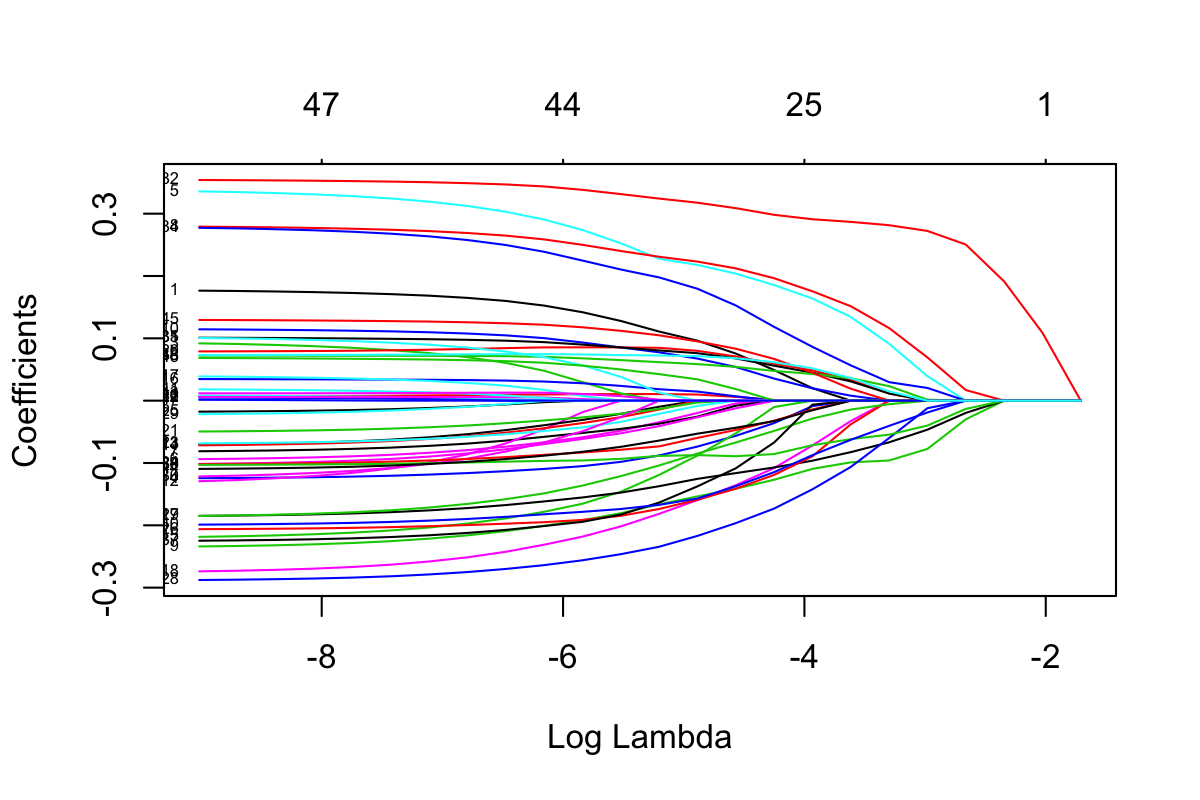
\includegraphics[width=1\linewidth]{./Generated_plots/CDlasso-1} 

}

\caption{Lasso plot of CD data}\label{fig:CDlasso}
\end{figure}

In Figure \ref{fig:CDlasso}, each curve corresponds to a variable
(e.g.~genus). It shows the path of its coefficient against different
\(log(\lambda)\) values. At each \(log(\lambda)\), the shown curves
indicate the number of nonzero coefficients. In the plot command, if
\textbf{label = T}, each curve will be annotated with variable index.

Once we have chosen the \(\lambda\) value, it is input in our new
wrapper function \emph{glmnet\_wrapper()}.

\begin{Shaded}
\begin{Highlighting}[]
\NormalTok{CD.lambda_clr =}\StringTok{ }\FloatTok{0.045}
\NormalTok{CD.results_clrlasso <-}\StringTok{ }\KeywordTok{glmnet_wrapper}\NormalTok{(}\DataTypeTok{Y =}\NormalTok{ CD.y.num, }\DataTypeTok{X =}\NormalTok{ CD.clrx, }\DataTypeTok{family =} \StringTok{'binomial'}\NormalTok{, }
                                      \DataTypeTok{lambda =}\NormalTok{ CD.lambda_clr)}
\NormalTok{CD.results_clrlasso}\OperatorTok{$}\NormalTok{numVarSelect}
\end{Highlighting}
\end{Shaded}

\begin{verbatim}
## [1] 11
\end{verbatim}

\begin{Shaded}
\begin{Highlighting}[]
\NormalTok{CD.results_clrlasso}\OperatorTok{$}\NormalTok{varSelect}
\end{Highlighting}
\end{Shaded}

\begin{verbatim}
##  [1] "g__Roseburia"                 "g__Eggerthella"              
##  [3] "g__Bacteroides"               "f__Peptostreptococcaceae_g__"
##  [5] "g__Dialister"                 "g__Streptococcus"            
##  [7] "g__Adlercreutzia"             "g__Aggregatibacter"          
##  [9] "o__Clostridiales_g__"         "g__Lachnospira"              
## [11] "o__Lactobacillales_g__"
\end{verbatim}

The method selects 11 genera with \(\lambda = 0.045\), and they are
listed in the object \textbf{CD.results\_clrlasso}.

\section{HFHS-Day1 data}\label{hfhs-day1-data-1}

The analysis on HFHS-Day1 data is as similar as CD data.

\begin{Shaded}
\begin{Highlighting}[]
\CommentTok{# CLR transformation}
\NormalTok{HFHS.z <-}\StringTok{ }\KeywordTok{log}\NormalTok{(HFHS.x)}
\NormalTok{HFHS.clrx <-}\StringTok{ }\KeywordTok{apply}\NormalTok{(HFHS.z, }\DecValTok{2}\NormalTok{, }\ControlFlowTok{function}\NormalTok{(x) x}\OperatorTok{-}\KeywordTok{rowMeans}\NormalTok{(HFHS.z))}
\end{Highlighting}
\end{Shaded}

\textbf{X} is centered log-ratio (CLR) transformed.

\begin{Shaded}
\begin{Highlighting}[]
\NormalTok{HFHS.y.num <-}\StringTok{ }\KeywordTok{as.numeric}\NormalTok{(HFHS.y)}
\end{Highlighting}
\end{Shaded}

\textbf{Y} is converted to a numeric vector.

\begin{Shaded}
\begin{Highlighting}[]
\NormalTok{HFHS.test_clrlasso <-}\StringTok{ }\KeywordTok{glmnet}\NormalTok{(}\DataTypeTok{x =}\NormalTok{ HFHS.clrx, }\DataTypeTok{y =}\NormalTok{ HFHS.y.num, }\DataTypeTok{family =} \StringTok{'binomial'}\NormalTok{)}
\KeywordTok{plot}\NormalTok{(HFHS.test_clrlasso, }\DataTypeTok{xvar =} \StringTok{'lambda'}\NormalTok{, }\DataTypeTok{label =}\NormalTok{ T)}
\end{Highlighting}
\end{Shaded}

\begin{figure}

{\centering 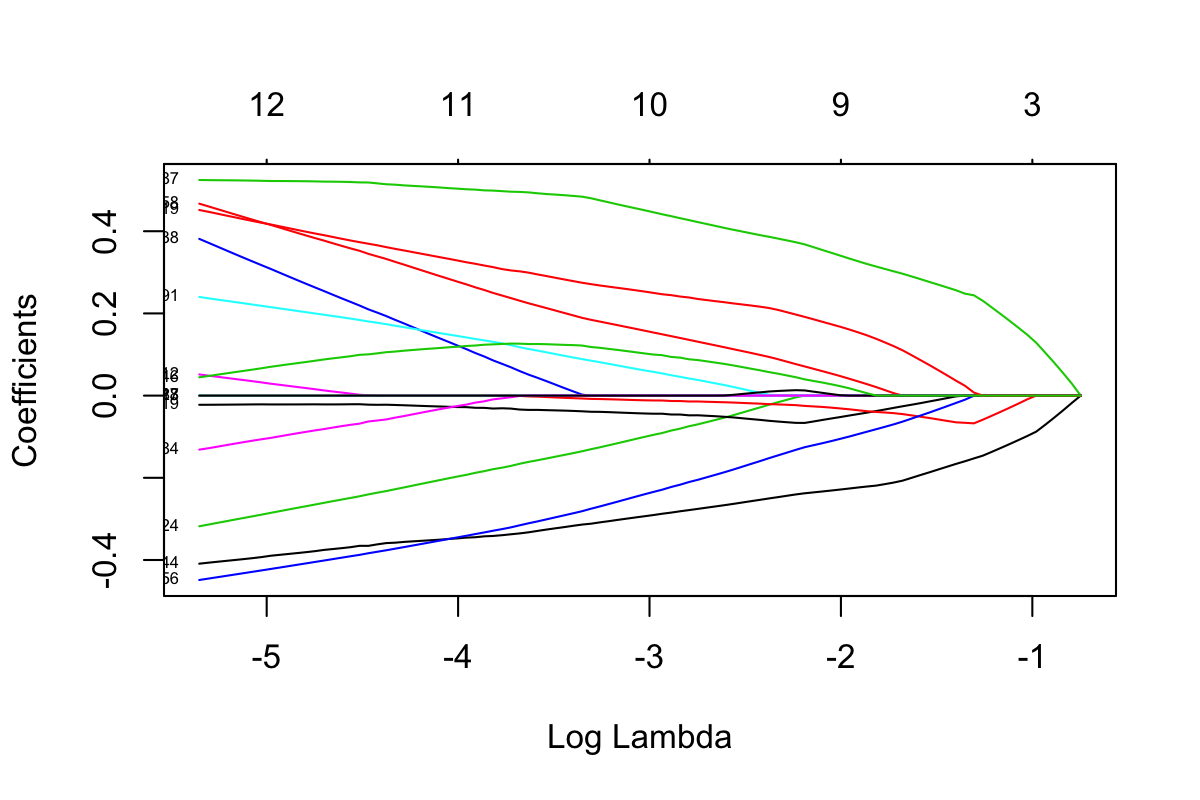
\includegraphics[width=1\linewidth]{./Generated_plots/HFHSlasso-1} 

}

\caption{Lasso plot of HFHS-Day1 data}\label{fig:HFHSlasso}
\end{figure}

The explanation of Figure \ref{fig:HFHSlasso} is the same as Figure
\ref{fig:CDlasso}.

Once we have chosen the \(\lambda\) value, we use function
\emph{glmnet\_wrapper()} with the same input as \emph{glmnet()} and
extra input \textbf{\(\lambda\)}.

\begin{Shaded}
\begin{Highlighting}[]
\NormalTok{HFHS.lambda_clr =}\StringTok{ }\FloatTok{0.03}
\NormalTok{HFHS.results_clrlasso <-}\StringTok{ }\KeywordTok{glmnet_wrapper}\NormalTok{(}\DataTypeTok{Y =}\NormalTok{ HFHS.y.num, }\DataTypeTok{X =}\NormalTok{ HFHS.clrx, }\DataTypeTok{family =} \StringTok{'binomial'}\NormalTok{, }
                                        \DataTypeTok{lambda =}\NormalTok{ HFHS.lambda_clr) }
\NormalTok{HFHS.results_clrlasso}\OperatorTok{$}\NormalTok{numVarSelect}
\end{Highlighting}
\end{Shaded}

\begin{verbatim}
## [1] 10
\end{verbatim}

\begin{Shaded}
\begin{Highlighting}[]
\NormalTok{HFHS.results_clrlasso}\OperatorTok{$}\NormalTok{varSelect}
\end{Highlighting}
\end{Shaded}

\begin{verbatim}
##  [1] "400599"  "192222"  "348038"  "401384"  "290253"  "261265"  "300851" 
##  [8] "462764"  "1108745" "265322"
\end{verbatim}

The method selects 10 OTUs with \(\lambda = 0.03\), and these OTUs are
listed in the object \textbf{HFHS.results\_clrlasso}.

We also extract the taxonomic information of these selected OTUs.

\begin{Shaded}
\begin{Highlighting}[]
\NormalTok{HFHS.tax_clrlasso <-}\StringTok{ }\NormalTok{HFHS.taxonomy[}\KeywordTok{which}\NormalTok{(}\KeywordTok{rownames}\NormalTok{(HFHS.taxonomy) }\OperatorTok\StringTok{ }
\StringTok{                                           }\NormalTok{HFHS.results_clrlasso}\OperatorTok{$}\NormalTok{varSelect), ]}
\KeywordTok{kable}\NormalTok{(HFHS.tax_clrlasso[ ,}\DecValTok{2}\OperatorTok{:}\DecValTok{6}\NormalTok{], }\DataTypeTok{booktabs =}\NormalTok{ T)}
\end{Highlighting}
\end{Shaded}

\begin{tabular}{llllll}
\toprule
  & Phylum & Class & Order & Family & Genus\\
\midrule
192222 & Bacteroidetes & Bacteroidia & Bacteroidales & Prevotellaceae & \\
290253 & Firmicutes & Clostridia & Clostridiales & Ruminococcaceae & Oscillospira\\
261265 & Firmicutes & Clostridia & Clostridiales & Lachnospiraceae & \\
1108745 & Firmicutes & Clostridia & Clostridiales & [Mogibacteriaceae] & \\
462764 & Firmicutes & Clostridia & Clostridiales & Ruminococcaceae & Ruminococcus\\
\addlinespace
265322 & Bacteroidetes & Bacteroidia & Bacteroidales & S24-7 & \\
400599 & Firmicutes & Clostridia & Clostridiales &  & \\
348038 & Bacteroidetes & Bacteroidia & Bacteroidales & S24-7 & \\
401384 & Firmicutes & Clostridia & Clostridiales & Ruminococcaceae & Oscillospira\\
300851 & Firmicutes & Clostridia & Clostridiales & Ruminococcaceae & Oscillospira\\
\bottomrule
\end{tabular}

\chapter{Selbal: selection of balances}\label{selbal}

selbal \citep{rivera2018balances} relies on the concept of compositional
balances, which is the balance between the abundances of two groups of
microbial species that is more associated with the response variable. We
also generated a wrapper function called \emph{selbal\_wrapper()}. It is
based on \emph{selbal()}, but provides additional outputs. All these
functions are uploaded via \textbf{functions.R}.

\section{CD data}\label{cd-data-2}

\begin{Shaded}
\begin{Highlighting}[]
\KeywordTok{class}\NormalTok{(CD.y)}
\end{Highlighting}
\end{Shaded}

\begin{verbatim}
## [1] "factor"
\end{verbatim}

\emph{selbal()} requires \textbf{Y} to be factor, as it will run
logistic regression with a binary outcomes. If \textbf{Y} is numeric,
\emph{selbal()} implements linear regression.

Besides input \textbf{Y} and \textbf{X}, we also need to decide how many
variables to select (\textbf{maxV}). The default performance measure
(\textbf{logit.acc}) to compute the correlation between \textbf{Y} and
balances is \textbf{AUC}, other opitions can be \textbf{``Dev''},
\textbf{``Rsq''} or \textbf{``Tjur''}.

\begin{Shaded}
\begin{Highlighting}[]
\CommentTok{# optimization criteria Deviance}
\NormalTok{CD.results_selbal <-}\StringTok{ }\KeywordTok{selbal_wrapper}\NormalTok{(}\DataTypeTok{Y =}\NormalTok{ CD.y, }\DataTypeTok{X =}\NormalTok{ CD.x, }\DataTypeTok{maxV =} \DecValTok{12}\NormalTok{, }\DataTypeTok{logit.acc =} \StringTok{'Dev'}\NormalTok{) }
\NormalTok{CD.results_selbal}\OperatorTok{$}\NormalTok{numVarSelect}
\end{Highlighting}
\end{Shaded}

\begin{verbatim}
## [1] 12
\end{verbatim}

\begin{Shaded}
\begin{Highlighting}[]
\NormalTok{CD.results_selbal}\OperatorTok{$}\NormalTok{varSelect}
\end{Highlighting}
\end{Shaded}

\begin{verbatim}
##  [1] "g__Roseburia"                 "g__Eggerthella"              
##  [3] "g__Dialister"                 "g__Streptococcus"            
##  [5] "f__Peptostreptococcaceae_g__" "g__Bacteroides"              
##  [7] "g__Aggregatibacter"           "g__Adlercreutzia"            
##  [9] "g__Dorea"                     "g__Oscillospira"             
## [11] "o__Clostridiales_g__"         "g__Blautia"
\end{verbatim}

The method selects 12 genera as we required.

\section{HFHS-Day1 data}\label{hfhs-day1-data-2}

The analysis on HFHS-Day1 data is as similar as CD data.

First, we need to check if \textbf{Y} is a factor.

\begin{Shaded}
\begin{Highlighting}[]
\KeywordTok{class}\NormalTok{(HFHS.y)}
\end{Highlighting}
\end{Shaded}

\begin{verbatim}
## [1] "factor"
\end{verbatim}

\begin{Shaded}
\begin{Highlighting}[]
\CommentTok{# optimization criteria Deviance}
\NormalTok{HFHS.results_selbal <-}\StringTok{ }\KeywordTok{selbal_wrapper}\NormalTok{(}\DataTypeTok{Y =}\NormalTok{ HFHS.y, }\DataTypeTok{X =}\NormalTok{ HFHS.x, }\DataTypeTok{maxV =} \DecValTok{2}\NormalTok{, }\DataTypeTok{logit.acc =} \StringTok{'Dev'}\NormalTok{) }
\NormalTok{HFHS.results_selbal}\OperatorTok{$}\NormalTok{numVarSelect}
\end{Highlighting}
\end{Shaded}

\begin{verbatim}
## [1] 2
\end{verbatim}

\begin{Shaded}
\begin{Highlighting}[]
\NormalTok{HFHS.results_selbal}\OperatorTok{$}\NormalTok{varSelect}
\end{Highlighting}
\end{Shaded}

\begin{verbatim}
## [1] "290253" "263479"
\end{verbatim}

The method selects 2 OTUs as required.

We also extract the taxonomic information of these selected OTUs.

\begin{Shaded}
\begin{Highlighting}[]
\NormalTok{HFHS.tax_selbal <-}\StringTok{ }\NormalTok{HFHS.taxonomy[}\KeywordTok{which}\NormalTok{(}\KeywordTok{rownames}\NormalTok{(HFHS.taxonomy) }\OperatorTok\StringTok{ }
\StringTok{                                         }\NormalTok{HFHS.results_selbal}\OperatorTok{$}\NormalTok{varSelect), ]}
\KeywordTok{kable}\NormalTok{(HFHS.tax_selbal[ ,}\DecValTok{2}\OperatorTok{:}\DecValTok{6}\NormalTok{], }\DataTypeTok{booktabs =}\NormalTok{ T)}
\end{Highlighting}
\end{Shaded}

\begin{tabular}{llllll}
\toprule
  & Phylum & Class & Order & Family & Genus\\
\midrule
290253 & Firmicutes & Clostridia & Clostridiales & Ruminococcaceae & Oscillospira\\
263479 & Bacteroidetes & Bacteroidia & Bacteroidales & S24-7 & \\
\bottomrule
\end{tabular}

\chapter{Concordance of variables selected by the three
methods}\label{comparison}

In this chapter, we are going to use different visualisation approaches
to display the variables selected by the three methods:

\begin{itemize}
\tightlist
\item
  \textbf{UpSet plot:} highlights overlap of the variables selected by
  the three methods.
\item
  \textbf{Selbal-like plot:} lists the selected variables and displays
  their discriminating ability with respect to sample groups.
\item
  \textbf{plotLoadings:} visualises the variable coefficients and sample
  groups each variable contributes to.
\item
  \textbf{Trajectory plot:} represents the rank of the variables
  selected by CoDA-lasso and CLR-lasso, and their corresponding
  regression coefficients
\item
  \textbf{GraPhlAn:} displays the taxonomic tree of selected variables
  (HFHS-Day1 data only).
\end{itemize}

\section{CD data}\label{cd-data-3}

\subsection{UpSetR}\label{upsetr}

UpSet is a visualisation technique for the quantitative analysis of sets
and their intersections \citep{lex2014upset}. Before we apply
\emph{upset()}, we take the list of variable vectors selected with the
three methods and convert them into a data frame compatible with
\emph{upset()} using \emph{fromList()}. We then assign different color
shcemes for each variable selection.

\begin{Shaded}
\begin{Highlighting}[]
\NormalTok{CD.select <-}\StringTok{ }\KeywordTok{list}\NormalTok{(}\DataTypeTok{CoDA_lasso =}\NormalTok{ CD.results_codalasso}\OperatorTok{$}\NormalTok{varSelect, }
                  \DataTypeTok{CLR_lasso =}\NormalTok{ CD.results_clrlasso}\OperatorTok{$}\NormalTok{varSelect, }
                  \DataTypeTok{selbal =}\NormalTok{ CD.results_selbal}\OperatorTok{$}\NormalTok{varSelect)}


\NormalTok{CD.select.upsetR <-}\StringTok{ }\KeywordTok{fromList}\NormalTok{(CD.select)}

\KeywordTok{upset}\NormalTok{(}\KeywordTok{as.data.frame}\NormalTok{(CD.select.upsetR), }\DataTypeTok{main.bar.color =} \StringTok{'gray36'}\NormalTok{, }
      \DataTypeTok{sets.bar.color =}\NormalTok{ color[}\KeywordTok{c}\NormalTok{(}\DecValTok{1}\OperatorTok{:}\DecValTok{2}\NormalTok{,}\DecValTok{5}\NormalTok{)], }\DataTypeTok{matrix.color =} \StringTok{'gray36'}\NormalTok{, }
      \DataTypeTok{order.by =} \StringTok{'freq'}\NormalTok{, }\DataTypeTok{empty.intersections =} \StringTok{'on'}\NormalTok{, }
      \DataTypeTok{queries =} \KeywordTok{list}\NormalTok{(}\KeywordTok{list}\NormalTok{(}\DataTypeTok{query =}\NormalTok{ intersects, }\DataTypeTok{params =} \KeywordTok{list}\NormalTok{(}\StringTok{'CoDA_lasso'}\NormalTok{), }
                          \DataTypeTok{color =}\NormalTok{ color[}\DecValTok{5}\NormalTok{], }\DataTypeTok{active =}\NormalTok{ T), }
                     \KeywordTok{list}\NormalTok{(}\DataTypeTok{query =}\NormalTok{ intersects, }\DataTypeTok{params =} \KeywordTok{list}\NormalTok{(}\StringTok{'CLR_lasso'}\NormalTok{), }
                          \DataTypeTok{color =}\NormalTok{ color[}\DecValTok{2}\NormalTok{], }\DataTypeTok{active =}\NormalTok{ T),}
                     \KeywordTok{list}\NormalTok{(}\DataTypeTok{query =}\NormalTok{ intersects, }\DataTypeTok{params =} \KeywordTok{list}\NormalTok{(}\StringTok{'selbal'}\NormalTok{), }
                          \DataTypeTok{color =}\NormalTok{ color[}\DecValTok{1}\NormalTok{], }\DataTypeTok{active =}\NormalTok{ T)))}
\end{Highlighting}
\end{Shaded}

\begin{figure}

{\centering 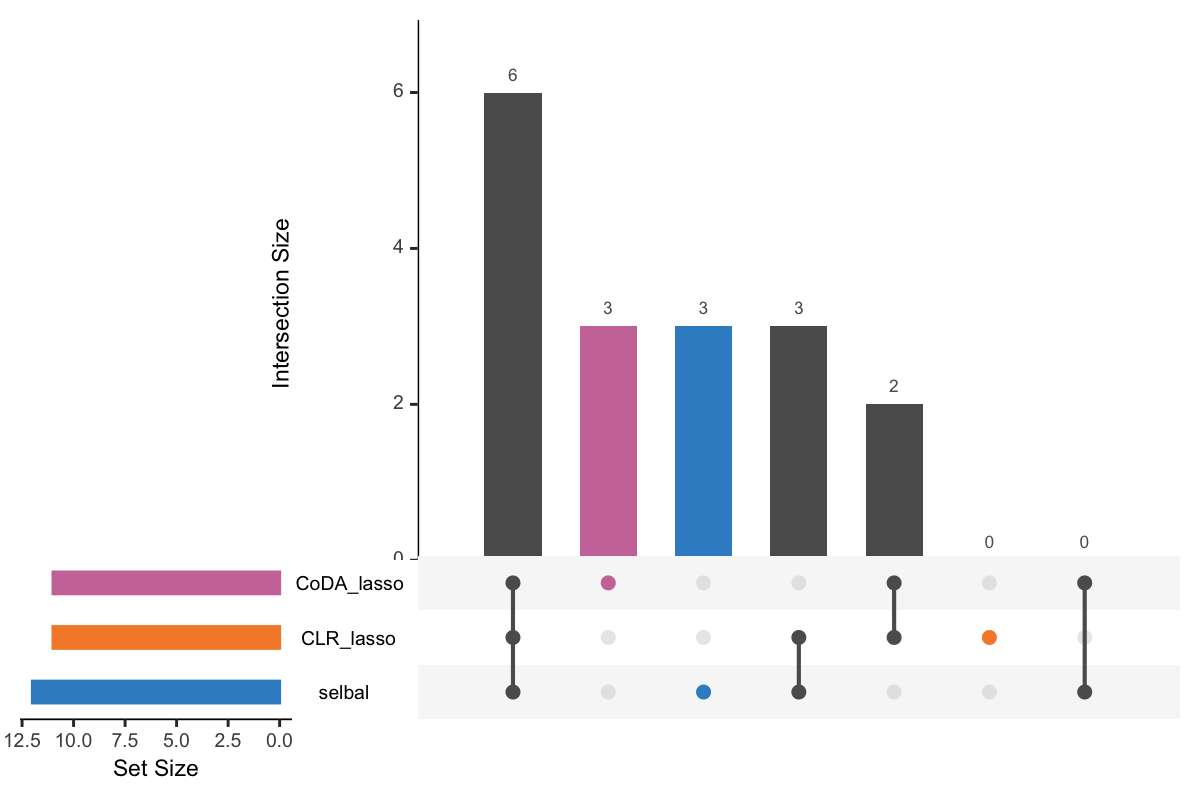
\includegraphics[width=1\linewidth]{./Generated_plots/upsetCD-1} 

}

\caption{UpSet plot showing overlap between variables selected with different methods.}\label{fig:upsetCD}
\end{figure}

In Figure \ref{fig:upsetCD}, the left bars show the number of variables
selected by each method. The right bar plot combined with the
scatterplot show different intersection situations and their aggregates.
For example, in the first column, three points are linked with one line,
and the intersection size of the bar is 6. This means that 6 variables
are selected by all these three methods. While in the second column, 3
variables are only selected by the method CoDA-lasso.

\subsection{Selbal-like plot}\label{selbal-like-plot}

Selbal-like plot is an extension of the plot proposed by
\citet{rivera2018balances}.

\begin{Shaded}
\begin{Highlighting}[]
\CommentTok{# CoDA_lasso}
\NormalTok{CD.coda_pos <-}\StringTok{ }\NormalTok{CD.results_codalasso}\OperatorTok{$}\NormalTok{posCoefSelect}
\NormalTok{CD.coda_neg <-}\StringTok{ }\NormalTok{CD.results_codalasso}\OperatorTok{$}\NormalTok{negCoefSelect}
\KeywordTok{selbal_like_plot}\NormalTok{(}\DataTypeTok{pos.names =} \KeywordTok{names}\NormalTok{(CD.coda_pos), }\DataTypeTok{neg.names =} \KeywordTok{names}\NormalTok{(CD.coda_neg), }
                 \DataTypeTok{Y =}\NormalTok{ CD.y, }\DataTypeTok{X =}\NormalTok{ CD.x)}
\end{Highlighting}
\end{Shaded}

\begin{figure}

{\centering 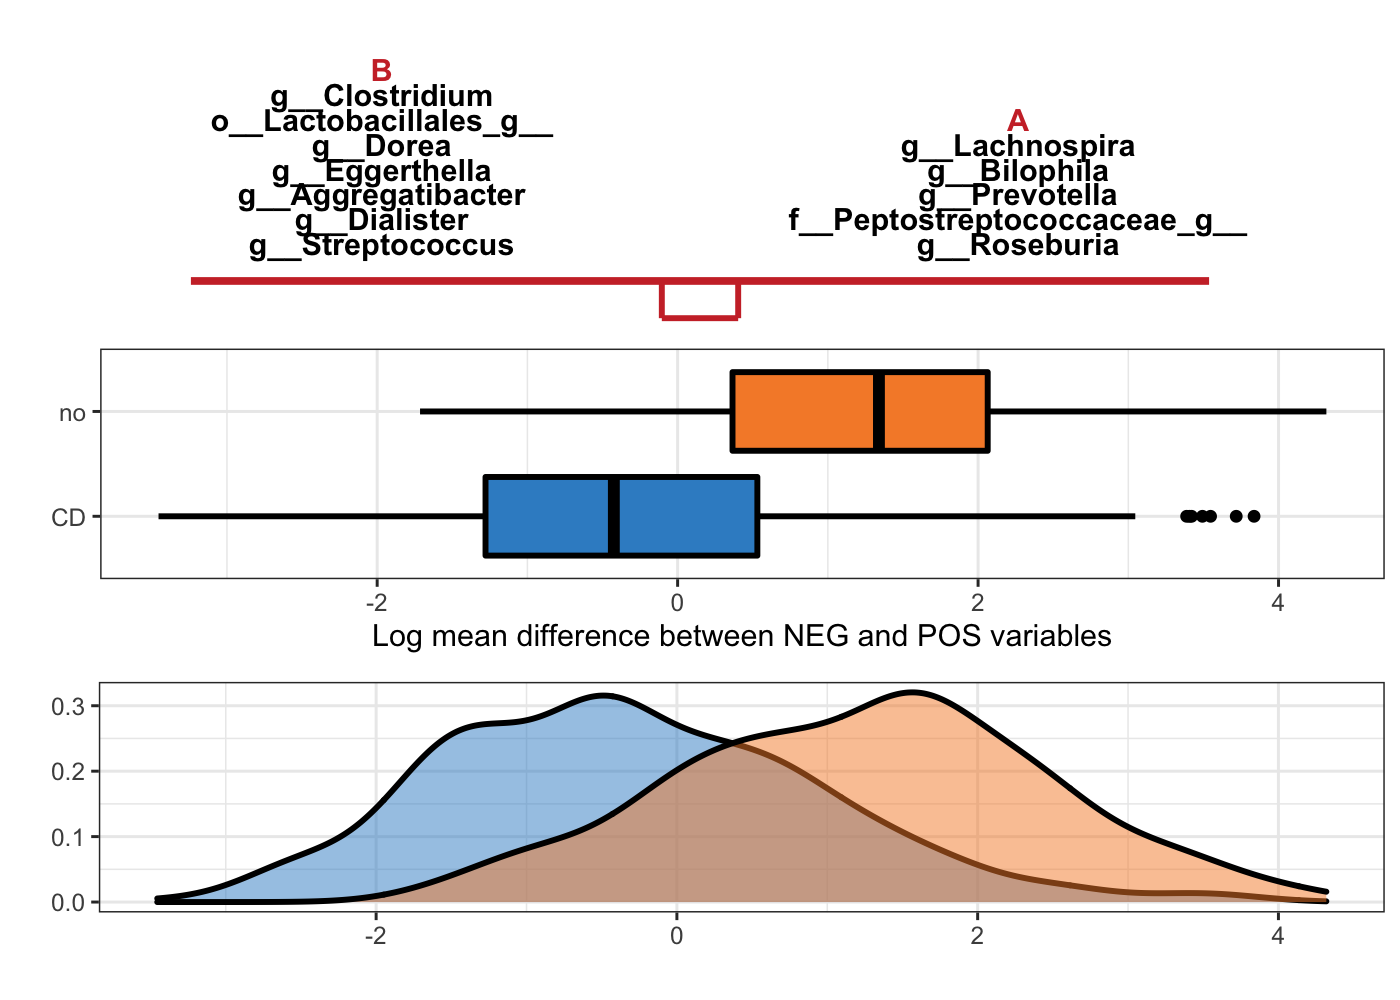
\includegraphics[width=1\linewidth]{./Generated_plots/codaCD-1} 

}

\caption{Selbal-like plot showing variables selected with method CoDA-lasso and the ability of these variables to discriminate CD and non-CD individuals.}\label{fig:codaCD}
\end{figure}

In Figure \ref{fig:codaCD}, the top left panel lists the selected
variable names with either negative or positive coefficients. The names
are ordered according to their importance (absolute coefficient values).
The top right panel is the Receiver Operating Characteristic (ROC) curve
based on generalised linear model:
\(g(E(Y)) = \beta_{0} + \beta_{1}logX_{1}+...+\beta_{p}logX_{p}\) with
\(p\) selected variables. The Area Under the Curve (AUC) is 0.822, which
indicates the ability to discriminate the sample groups. The bottom left
boxplot is based on the log mean difference between negative and
positive variables:
\(\frac{1}{p_{+}}\sum_{i=1}^{p_{+}}logX_{i} - \frac{1}{p_{-}}\sum_{j=1}^{p_{-}}logX_{j}\).
This log mean difference is calculated for each sample as a balance
score, because it is proportionally equal to the balance mentioned in
\citep{rivera2018balances}. The bottom right density plots represent the
distributions of the log mean difference scores for CD and non-CD
individuals.

\begin{Shaded}
\begin{Highlighting}[]
\CommentTok{# CLR_lasso}
\NormalTok{CD.clr_pos <-}\StringTok{ }\NormalTok{CD.results_clrlasso}\OperatorTok{$}\NormalTok{posCoefSelect}
\NormalTok{CD.clr_neg <-}\StringTok{ }\NormalTok{CD.results_clrlasso}\OperatorTok{$}\NormalTok{negCoefSelect}
\KeywordTok{selbal_like_plot}\NormalTok{(}\DataTypeTok{pos.names =} \KeywordTok{names}\NormalTok{(CD.clr_pos), }\DataTypeTok{neg.names =} \KeywordTok{names}\NormalTok{(CD.clr_neg), }
                 \DataTypeTok{Y =}\NormalTok{ CD.y, }\DataTypeTok{X =}\NormalTok{ CD.x)}
\end{Highlighting}
\end{Shaded}

\begin{figure}

{\centering 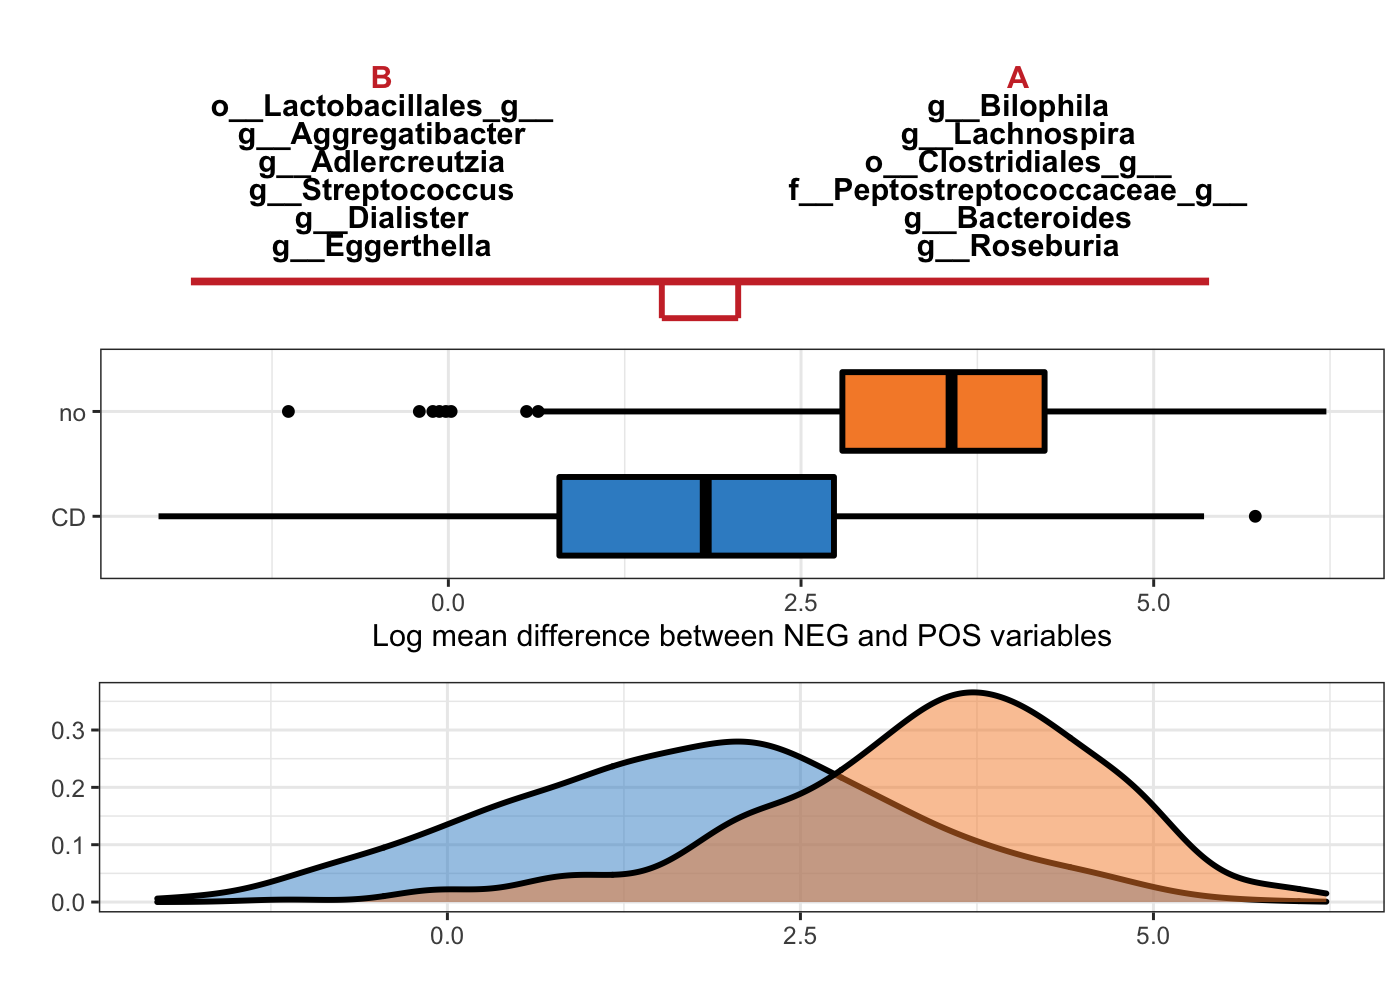
\includegraphics[width=1\linewidth]{./Generated_plots/clrCD-1} 

}

\caption{Selbal-like plot showing variables selected with method CLR-lasso and the ability of these variables to discriminate CD and non-CD individuals.}\label{fig:clrCD}
\end{figure}

The interpretation of Figure \ref{fig:clrCD} is the same as Figure
\ref{fig:codaCD}, but with variables selected with method CLR-lasso.

\begin{Shaded}
\begin{Highlighting}[]
\CommentTok{# selbal}
\NormalTok{CD.selbal_pos <-}\StringTok{ }\NormalTok{CD.results_selbal}\OperatorTok{$}\NormalTok{posVarSelect}
\NormalTok{CD.selbal_neg <-}\StringTok{ }\NormalTok{CD.results_selbal}\OperatorTok{$}\NormalTok{negVarSelect}
\KeywordTok{selbal_like_plot}\NormalTok{(}\DataTypeTok{pos.names =}\NormalTok{ CD.selbal_pos, }\DataTypeTok{neg.names =}\NormalTok{ CD.selbal_neg, }\DataTypeTok{Y =}\NormalTok{ CD.y, }
                 \DataTypeTok{selbal =} \OtherTok{TRUE}\NormalTok{, }\DataTypeTok{FINAL.BAL =}\NormalTok{ CD.results_selbal}\OperatorTok{$}\NormalTok{finalBal)}
\end{Highlighting}
\end{Shaded}

\begin{figure}

{\centering 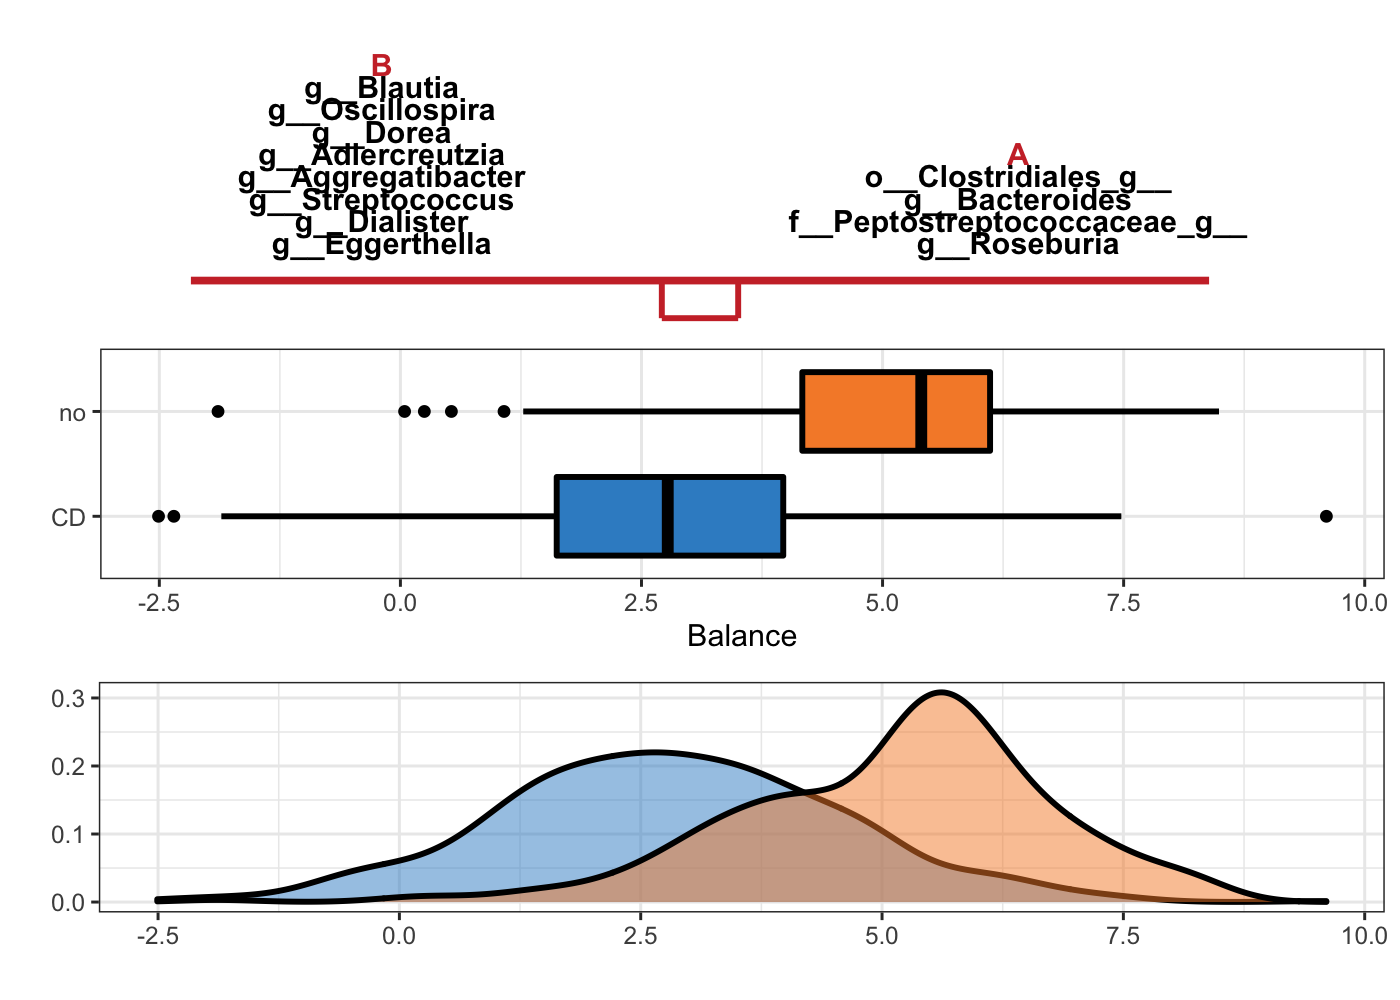
\includegraphics[width=1\linewidth]{./Generated_plots/selbalCD-1} 

}

\caption{Selbal plot showing variables selected with method selbal and the ability of these variables to discriminate CD and non-CD individuals.}\label{fig:selbalCD}
\end{figure}

In Figure \ref{fig:selbalCD}, for the selbal method, the two groups of
variables that form the global balance are specified at the top of the
plot. They are equally important. The box plot represents the
distribution of the balance scores for CD and non-CD individuals. The
right part of the figure contains the ROC curve
(\(g(E(Y)) = \beta_{0} + \beta_{1}B(Den,Num)\)) with its AUC value
(0.841, higher than other methods) and the density curve for each group.

\subsection{plotLoadings}\label{plotloadings}

As all these above plots do not visualise the coefficients of the
selected variables, we then apply a modified plotLoadings
\citep{rohart2017mint} to display the coefficients.

\begin{Shaded}
\begin{Highlighting}[]
\CommentTok{# CoDA_lasso}
\NormalTok{CD.coda_coef <-}\StringTok{ }\NormalTok{CD.results_codalasso}\OperatorTok{$}\NormalTok{coefficientsSelect}
\NormalTok{CD.coda_data <-}\StringTok{ }\NormalTok{CD.x[ ,CD.results_codalasso}\OperatorTok{$}\NormalTok{varSelect]}

\NormalTok{CD.coda.plotloadings <-}\StringTok{ }\KeywordTok{plotcoefficients}\NormalTok{(}\DataTypeTok{coef =}\NormalTok{ CD.coda_coef, }
                                         \DataTypeTok{data =}\NormalTok{ CD.coda_data, }
                                         \DataTypeTok{Y =}\NormalTok{ CD.y, }
                                         \DataTypeTok{title =} \StringTok{'Coefficients of CoDA-lasso on CD data'}\NormalTok{)}
\end{Highlighting}
\end{Shaded}

\begin{figure}

{\centering 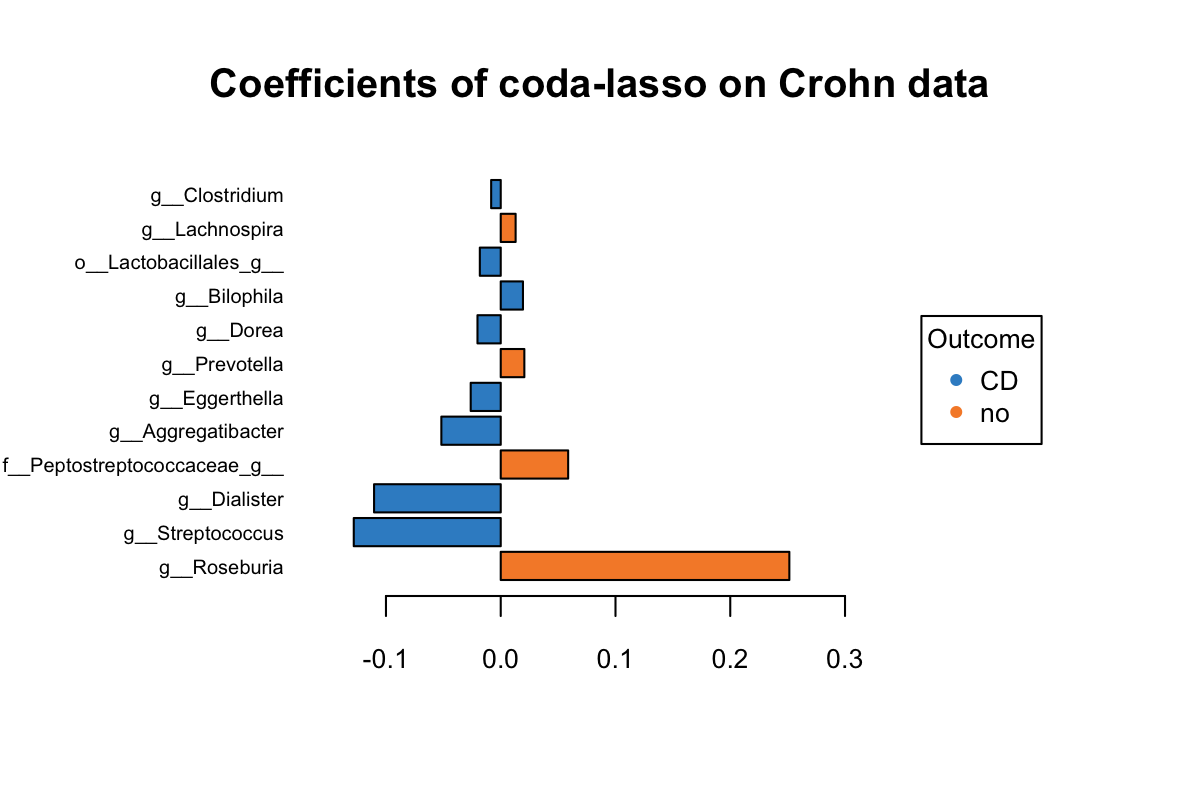
\includegraphics[width=1\linewidth]{./Generated_plots/loadcodaCD-1} 

}

\caption{The plotLoadings of selected variables with CoDA-lasso.}\label{fig:loadcodaCD}
\end{figure}

Figure \ref{fig:loadcodaCD} shows that the taxa colored in orange are
more abundant in non-CD samples relative to CD samples (e.g.
\emph{Roseburia}), while the blue ones are more abundant in CD samples
relative to non-CD samples (e.g. \emph{Dialister}). It is based on their
mean per group (CD vs.~non-CDs). The bar indicates the coefficient. As
we can see, several taxa are more abundant in non-CD group, but with a
negative coefficient. It means this model is not optimal at some extent.

\begin{Shaded}
\begin{Highlighting}[]
\CommentTok{# CLR_lasso}
\NormalTok{CD.clr_coef <-}\StringTok{ }\NormalTok{CD.results_clrlasso}\OperatorTok{$}\NormalTok{coefficientsSelect}
\NormalTok{CD.clr_data <-}\StringTok{ }\NormalTok{CD.x[ ,CD.results_clrlasso}\OperatorTok{$}\NormalTok{varSelect]}
\NormalTok{CD.clr.plotloadings <-}\StringTok{ }\KeywordTok{plotcoefficients}\NormalTok{(}\DataTypeTok{coef =}\NormalTok{ CD.clr_coef, }
                                        \DataTypeTok{data =}\NormalTok{ CD.clr_data, }
                                        \DataTypeTok{Y =}\NormalTok{ CD.y, }
                                        \DataTypeTok{title =} \StringTok{'Coefficients of clr-lasso on CD data'}\NormalTok{)}
\end{Highlighting}
\end{Shaded}

\begin{figure}

{\centering 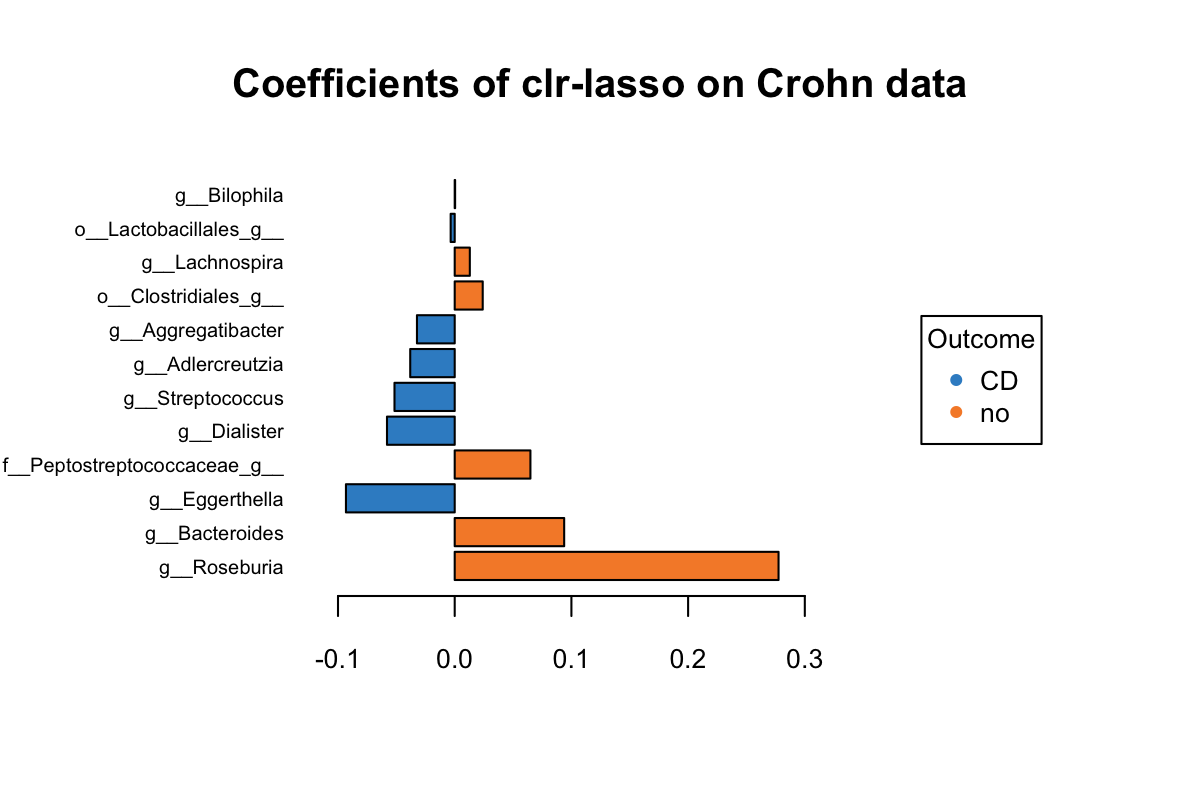
\includegraphics[width=1\linewidth]{./Generated_plots/loadclrCD-1} 

}

\caption{The plotLoadings of selected variables with CLR-lasso.}\label{fig:loadclrCD}
\end{figure}

The interpretation of Figure \ref{fig:loadclrCD} is the same as Figure
\ref{fig:loadcodaCD}. From Figure \ref{fig:loadclrCD}, all the selected
variables that more abundant in non-CD samples are assigned with
positive coefficients. It means CLR-lasso seems more optimal than
CoDA-lasso. Both \emph{Roseburia} and \emph{Peptostreptococcaceae} are
selected by CoDA-lasso and CLR-lasso that are more abundant in non-CD
group. Although both \emph{Eggerthella} and \emph{Dialister} are also
selected by two methods, but with very different coefficient rank.

\subsection{Trajectory plots}\label{trajectory-plots}

To visualise the change of variable coefficients and their ranks in the
selection between different methods, we introduce trajectory plots.

\begin{Shaded}
\begin{Highlighting}[]
\KeywordTok{TRAJ_plot}\NormalTok{(}\DataTypeTok{selectVar_coef_method1 =}\NormalTok{ CD.coda_coef, }\DataTypeTok{selectVar_coef_method2 =}\NormalTok{ CD.clr_coef, }
          \DataTypeTok{selectMethods =} \KeywordTok{c}\NormalTok{(}\StringTok{'CoDA-lasso'}\NormalTok{, }\StringTok{'CLR-lasso'}\NormalTok{))}
\end{Highlighting}
\end{Shaded}

\begin{figure}

{\centering 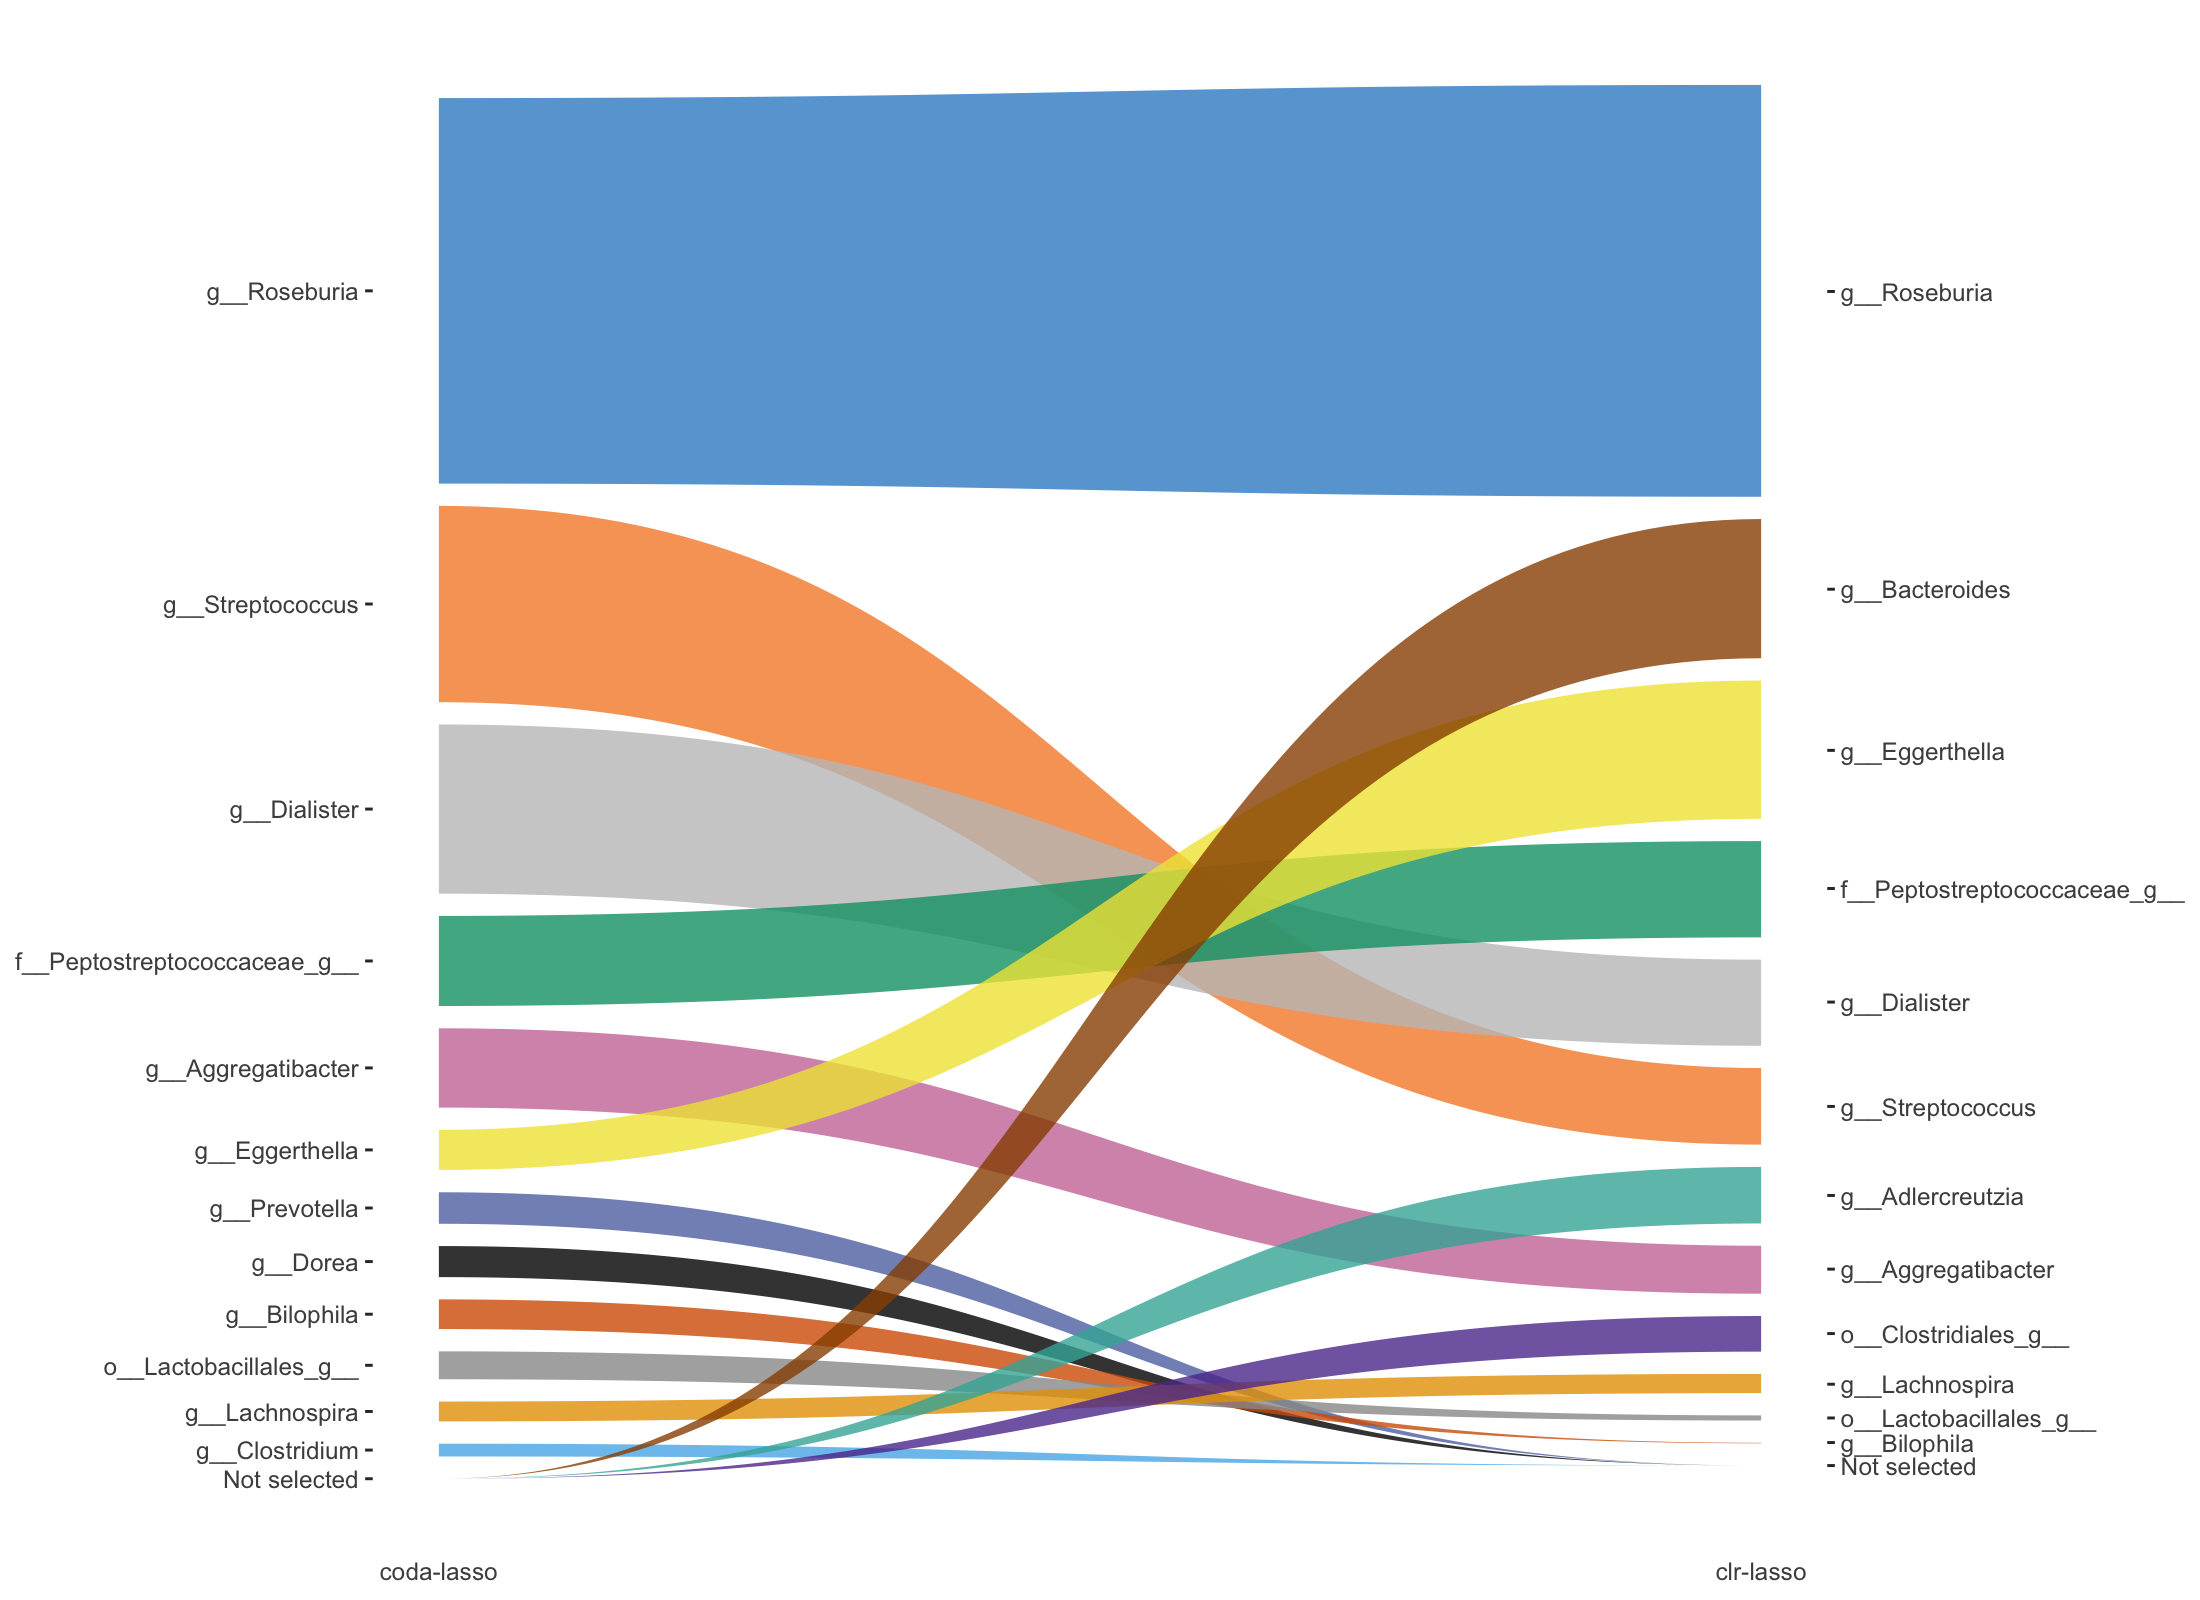
\includegraphics[width=1\linewidth]{./Generated_plots/trajCD-1} 

}

\caption{Trajectory plots of selected variables from both CoDA-lasso and CLR-lasso in CD data.}\label{fig:trajCD}
\end{figure}

Figure \ref{fig:trajCD} shows the selected variables ordered by their
rank in the selection (according to their coefficient absolute values)
between CoDA-lasso and CLR-lasso, with the thickness of the lines
representing the coefficient absolute values.

In this plot, it is easy to visualise the rank change of each selected
variable between CoDA-lasso and CLR-lasso selection. For example, the
rank of \emph{Dialister} is lower in CLR-lasso compared to CoDA-lasso.
Moreover, it is also easy to detect the variables (e.g.
\emph{Bacteroides}) that are selected by one method (e.g.~CLR-lasso)
with high coefficient rank, but not selected by the other method
(e.g.~CoDA-lasso).

\section{HFHS-Day1 data}\label{hfhs-day1-data-3}

\subsection{UpSetR}\label{upsetr-1}

\begin{Shaded}
\begin{Highlighting}[]
\NormalTok{HFHS.select <-}\StringTok{ }\KeywordTok{list}\NormalTok{(}\DataTypeTok{CoDA_lasso =}\NormalTok{ HFHS.results_codalasso}\OperatorTok{$}\NormalTok{varSelect, }
                  \DataTypeTok{CLR_lasso =}\NormalTok{ HFHS.results_clrlasso}\OperatorTok{$}\NormalTok{varSelect, }
                  \DataTypeTok{selbal =}\NormalTok{ HFHS.results_selbal}\OperatorTok{$}\NormalTok{varSelect)}

\NormalTok{HFHS.select.upsetR <-}\StringTok{ }\KeywordTok{fromList}\NormalTok{(HFHS.select)}

\KeywordTok{upset}\NormalTok{(}\KeywordTok{as.data.frame}\NormalTok{(HFHS.select.upsetR), }\DataTypeTok{main.bar.color =} \StringTok{'gray36'}\NormalTok{, }
      \DataTypeTok{sets.bar.color =}\NormalTok{ color[}\KeywordTok{c}\NormalTok{(}\DecValTok{5}\NormalTok{,}\DecValTok{2}\NormalTok{,}\DecValTok{1}\NormalTok{)], }\DataTypeTok{matrix.color =} \StringTok{'gray36'}\NormalTok{, }
      \DataTypeTok{order.by =} \StringTok{'freq'}\NormalTok{, }\DataTypeTok{empty.intersections =} \StringTok{'on'}\NormalTok{, }
      \DataTypeTok{queries =} \KeywordTok{list}\NormalTok{(}\KeywordTok{list}\NormalTok{(}\DataTypeTok{query =}\NormalTok{ intersects, }\DataTypeTok{params =} \KeywordTok{list}\NormalTok{(}\StringTok{'CoDA_lasso'}\NormalTok{), }
                          \DataTypeTok{color =}\NormalTok{ color[}\DecValTok{5}\NormalTok{], }\DataTypeTok{active =}\NormalTok{ T), }
                     \KeywordTok{list}\NormalTok{(}\DataTypeTok{query =}\NormalTok{ intersects, }\DataTypeTok{params =} \KeywordTok{list}\NormalTok{(}\StringTok{'CLR_lasso'}\NormalTok{), }
                          \DataTypeTok{color =}\NormalTok{ color[}\DecValTok{2}\NormalTok{], }\DataTypeTok{active =}\NormalTok{ T),}
                     \KeywordTok{list}\NormalTok{(}\DataTypeTok{query =}\NormalTok{ intersects, }\DataTypeTok{params =} \KeywordTok{list}\NormalTok{(}\StringTok{'selbal'}\NormalTok{), }
                          \DataTypeTok{color =}\NormalTok{ color[}\DecValTok{1}\NormalTok{], }\DataTypeTok{active =}\NormalTok{ T)))}
\end{Highlighting}
\end{Shaded}

\begin{figure}

{\centering 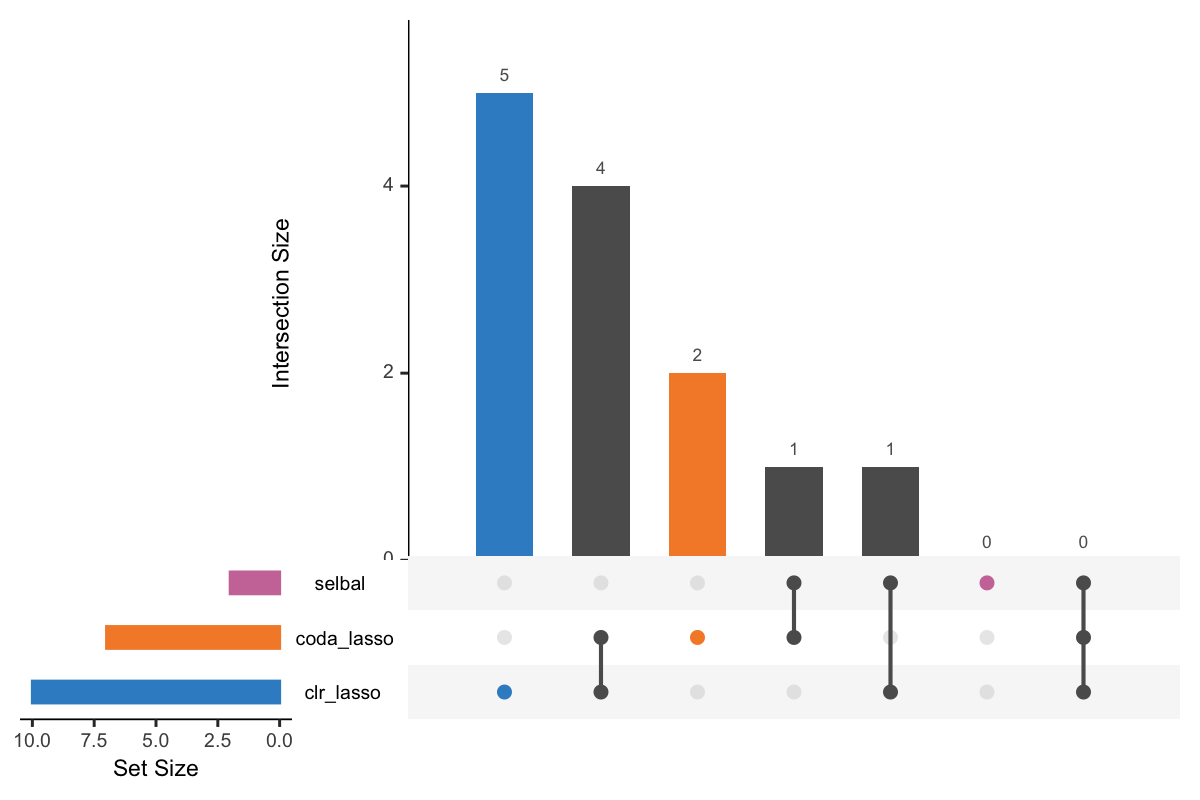
\includegraphics[width=1\linewidth]{./Generated_plots/upsetHFHS-1} 

}

\caption{UpSet plot showing overlap between variables selected with different methods.}\label{fig:upsetHFHS}
\end{figure}

Figure \ref{fig:upsetHFHS} shows that 5 OTUs are only selected with
CoDA-lasso, 5 OTUs are selected both with CoDA-lasso and CLR-lasso, 4
OTUs are only selected with CLR-lasso, 1 OTUs is selected with both
CLR-lasso and selbal, and 1 is selected both with CoDA-lasso and selbal.
Among three methods, CoDA-lasso selected the most OTUs and selbal the
least.

\subsection{Selbal-like plot}\label{selbal-like-plot-1}

\begin{Shaded}
\begin{Highlighting}[]
\CommentTok{# CoDA_lasso}
\NormalTok{HFHS.coda_pos <-}\StringTok{ }\NormalTok{HFHS.results_codalasso}\OperatorTok{$}\NormalTok{posCoefSelect}
\NormalTok{HFHS.coda_neg <-}\StringTok{ }\NormalTok{HFHS.results_codalasso}\OperatorTok{$}\NormalTok{negCoefSelect}
\KeywordTok{selbal_like_plot}\NormalTok{(}\DataTypeTok{pos.names =} \KeywordTok{names}\NormalTok{(HFHS.coda_pos), }\DataTypeTok{neg.names =} \KeywordTok{names}\NormalTok{(HFHS.coda_neg), }
                 \DataTypeTok{Y =}\NormalTok{ HFHS.y, }\DataTypeTok{X =}\NormalTok{ HFHS.x, }\DataTypeTok{OTU =}\NormalTok{ T, }\DataTypeTok{taxa =}\NormalTok{ HFHS.taxonomy)}
\end{Highlighting}
\end{Shaded}

\begin{figure}

{\centering 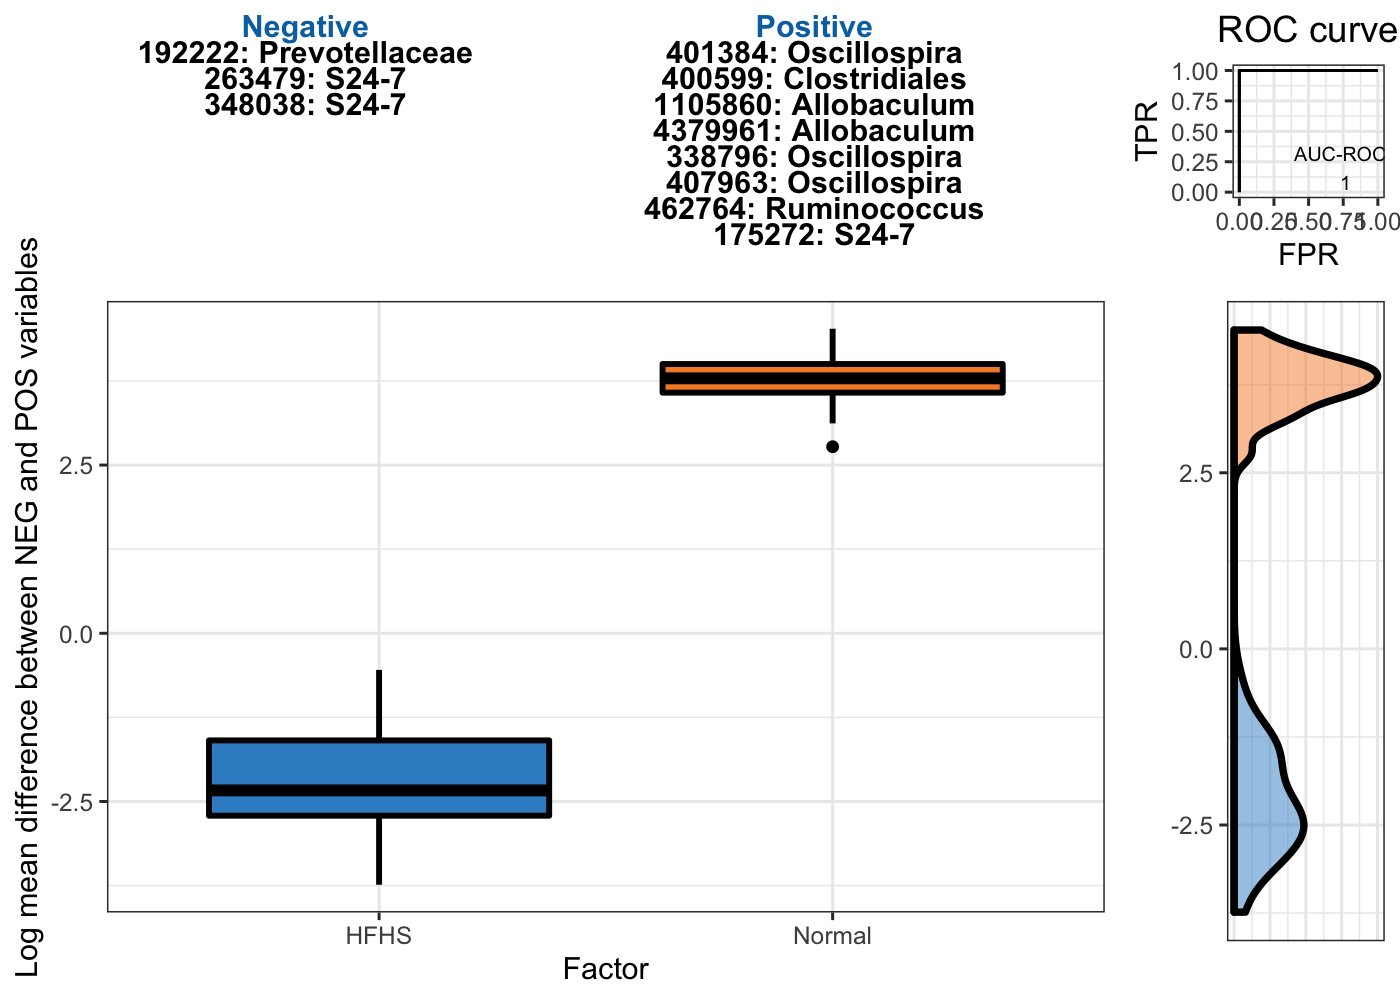
\includegraphics[width=1\linewidth]{./Generated_plots/unnamed-chunk-24-1} 

}

\caption{Selbal-like plot showing variables selected with method CoDA-lasso and the ability of these variables to discriminate HFHS and normal individuals.}\label{fig:unnamed-chunk-24}
\end{figure}

\textbf{Note:} \emph{S24-7} is a family from order \emph{Bacteroidales}.

\begin{Shaded}
\begin{Highlighting}[]
\CommentTok{# CLR_lasso}
\NormalTok{HFHS.clr_pos <-}\StringTok{ }\NormalTok{HFHS.results_clrlasso}\OperatorTok{$}\NormalTok{posCoefSelect}
\NormalTok{HFHS.clr_neg <-}\StringTok{ }\NormalTok{HFHS.results_clrlasso}\OperatorTok{$}\NormalTok{negCoefSelect}
\KeywordTok{selbal_like_plot}\NormalTok{(}\DataTypeTok{pos.names =} \KeywordTok{names}\NormalTok{(HFHS.clr_pos), }\DataTypeTok{neg.names =} \KeywordTok{names}\NormalTok{(HFHS.clr_neg), }
                 \DataTypeTok{Y =}\NormalTok{ HFHS.y, }\DataTypeTok{X =}\NormalTok{ HFHS.x, }\DataTypeTok{OTU =}\NormalTok{ T, }\DataTypeTok{taxa =}\NormalTok{ HFHS.taxonomy)}
\end{Highlighting}
\end{Shaded}

\begin{figure}

{\centering 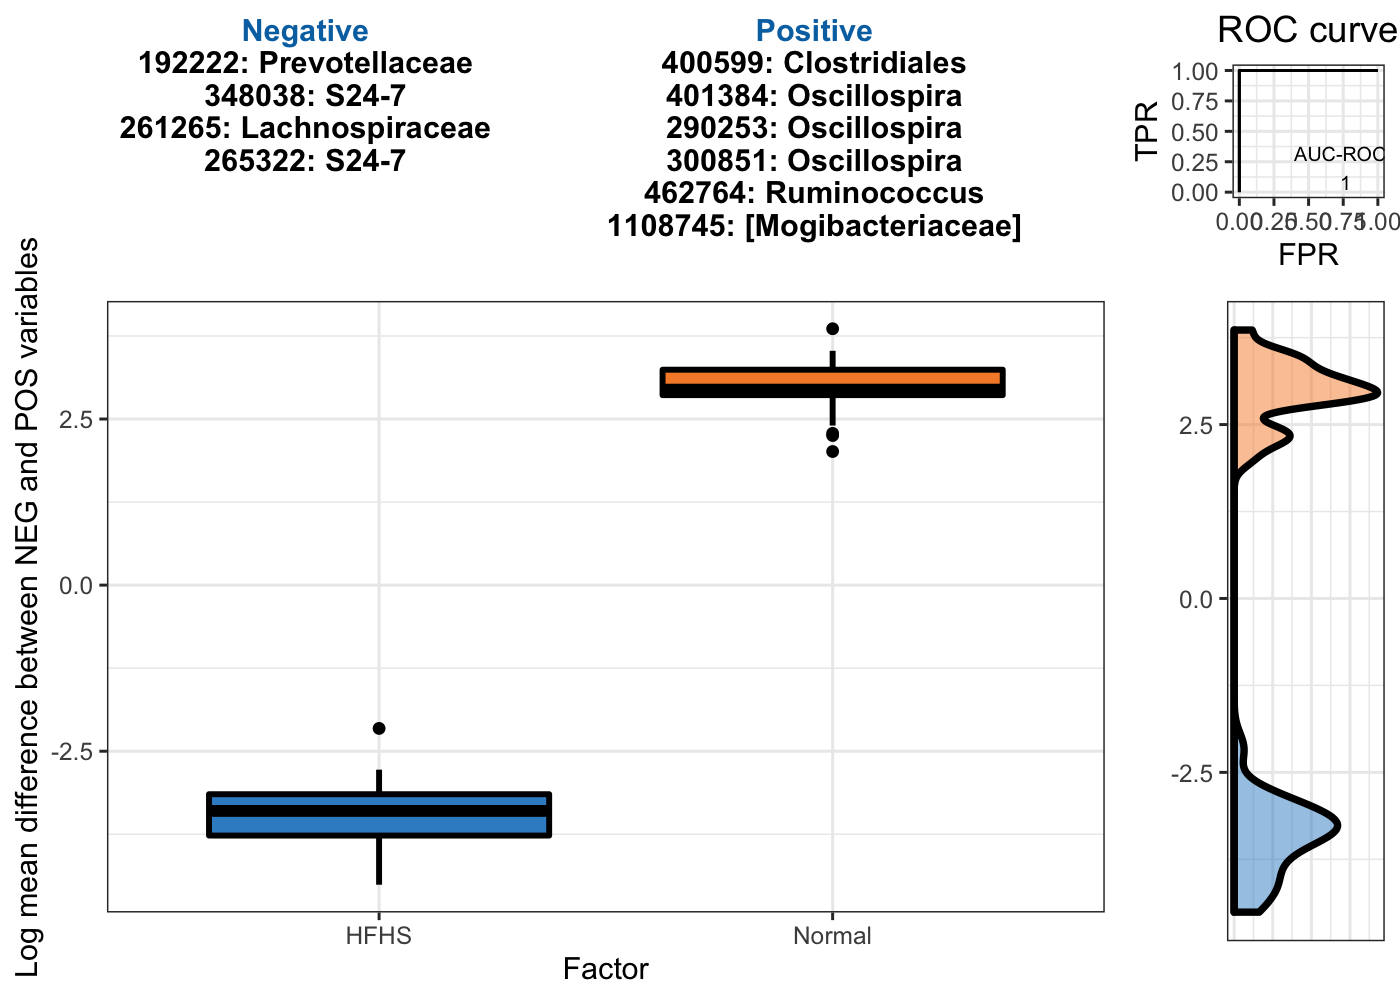
\includegraphics[width=1\linewidth]{./Generated_plots/unnamed-chunk-25-1} 

}

\caption{Selbal-like plot showing variables selected with method CLR-lasso and the ability of these variables to discriminate HFHS and normal individuals.}\label{fig:unnamed-chunk-25}
\end{figure}

\begin{Shaded}
\begin{Highlighting}[]
\CommentTok{# selbal}
\NormalTok{HFHS.selbal_pos <-}\StringTok{ }\NormalTok{HFHS.results_selbal}\OperatorTok{$}\NormalTok{posVarSelect}
\NormalTok{HFHS.selbal_neg <-}\StringTok{ }\NormalTok{HFHS.results_selbal}\OperatorTok{$}\NormalTok{negVarSelect}
\KeywordTok{selbal_like_plot}\NormalTok{(}\DataTypeTok{pos.names =}\NormalTok{ HFHS.selbal_pos, }\DataTypeTok{neg.names =}\NormalTok{ HFHS.selbal_neg, }\DataTypeTok{Y =}\NormalTok{ HFHS.y, }
                 \DataTypeTok{selbal =} \OtherTok{TRUE}\NormalTok{, }\DataTypeTok{FINAL.BAL =}\NormalTok{ HFHS.results_selbal}\OperatorTok{$}\NormalTok{finalBal, }
                 \DataTypeTok{OTU =}\NormalTok{ T, }\DataTypeTok{taxa =}\NormalTok{ HFHS.taxonomy)}
\end{Highlighting}
\end{Shaded}

\begin{figure}

{\centering 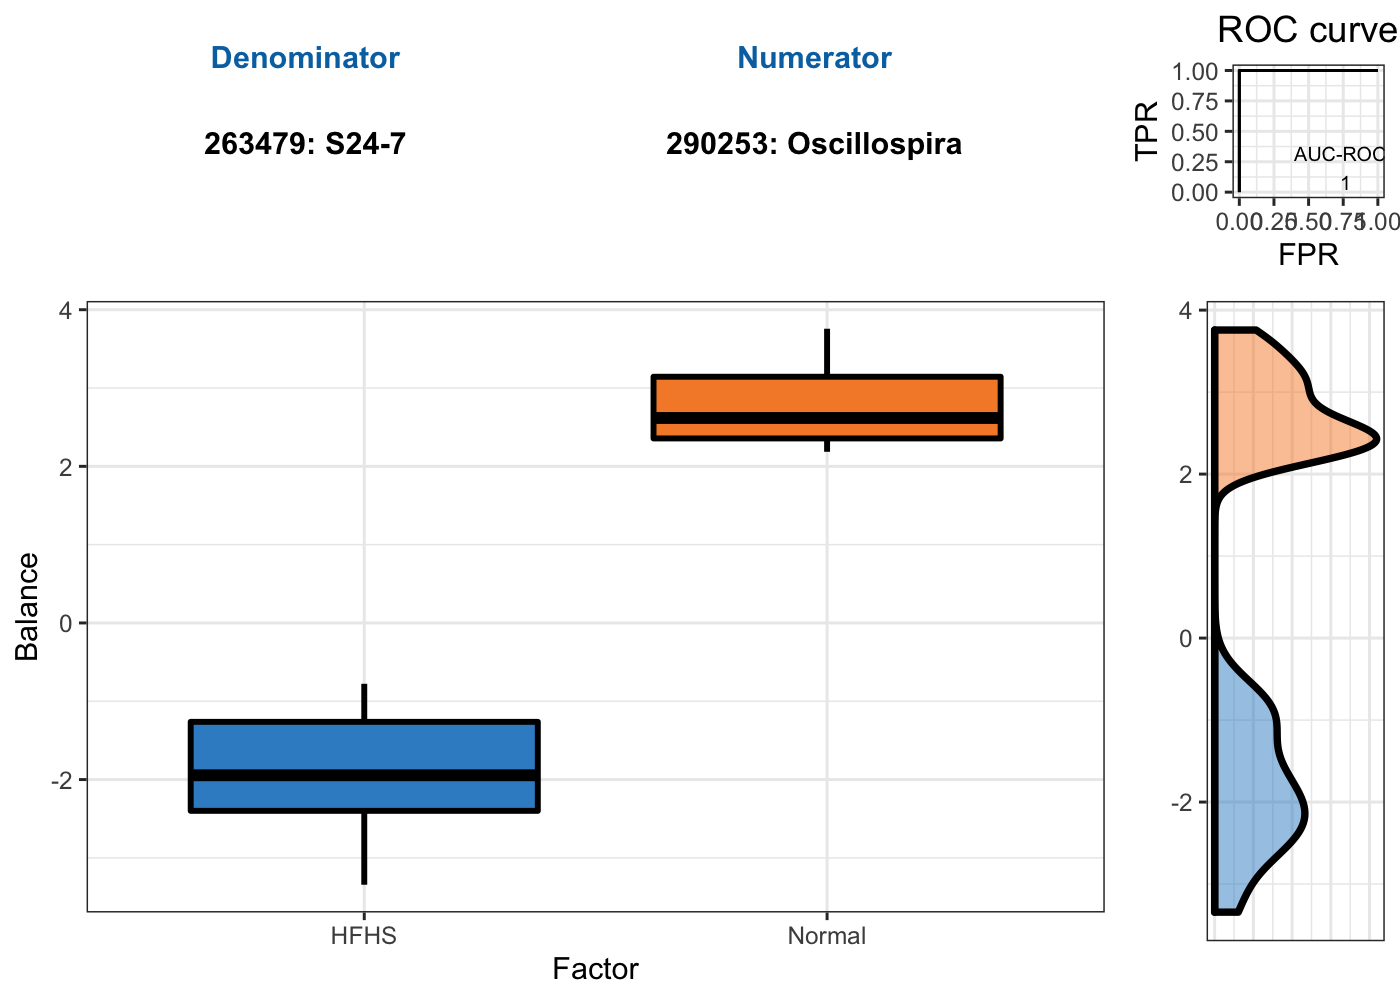
\includegraphics[width=1\linewidth]{./Generated_plots/unnamed-chunk-26-1} 

}

\caption{Selbal plot showing variables selected with methd selbal and the ability of these variables to discriminate HFHS and normal individuals.}\label{fig:unnamed-chunk-26}
\end{figure}

These plots show that the variables selected from three different
methods all have a maximum discrimination (AUC = 1) between HFHS samples
and normal ones. Among these methods, selbal only needs two OTUs to
build a balance, it also means the association between microbiome
composition and diet is very strong.

\subsection{plotLoadings}\label{plotloadings-1}

\begin{Shaded}
\begin{Highlighting}[]
\CommentTok{# CoDA_lasso}
\NormalTok{HFHS.coda_coef <-}\StringTok{ }\NormalTok{HFHS.results_codalasso}\OperatorTok{$}\NormalTok{coefficientsSelect}
\NormalTok{HFHS.coda_data <-}\StringTok{ }\NormalTok{HFHS.x[ ,HFHS.results_codalasso}\OperatorTok{$}\NormalTok{varSelect]}

\NormalTok{HFHS.coda.plotloadings <-}\StringTok{ }\KeywordTok{plotcoefficients}\NormalTok{(}\DataTypeTok{coef =}\NormalTok{ HFHS.coda_coef, }
                                           \DataTypeTok{data =}\NormalTok{ HFHS.coda_data, }
                                           \DataTypeTok{Y =}\NormalTok{ HFHS.y, }
                                           \DataTypeTok{title =} \StringTok{'Coefficients of CoDA-lasso on HFHS-Day1 data'}\NormalTok{,}
                                           \DataTypeTok{OTU =}\NormalTok{ T,}
                                           \DataTypeTok{taxa =}\NormalTok{ HFHS.taxonomy)}
\end{Highlighting}
\end{Shaded}

\begin{figure}

{\centering 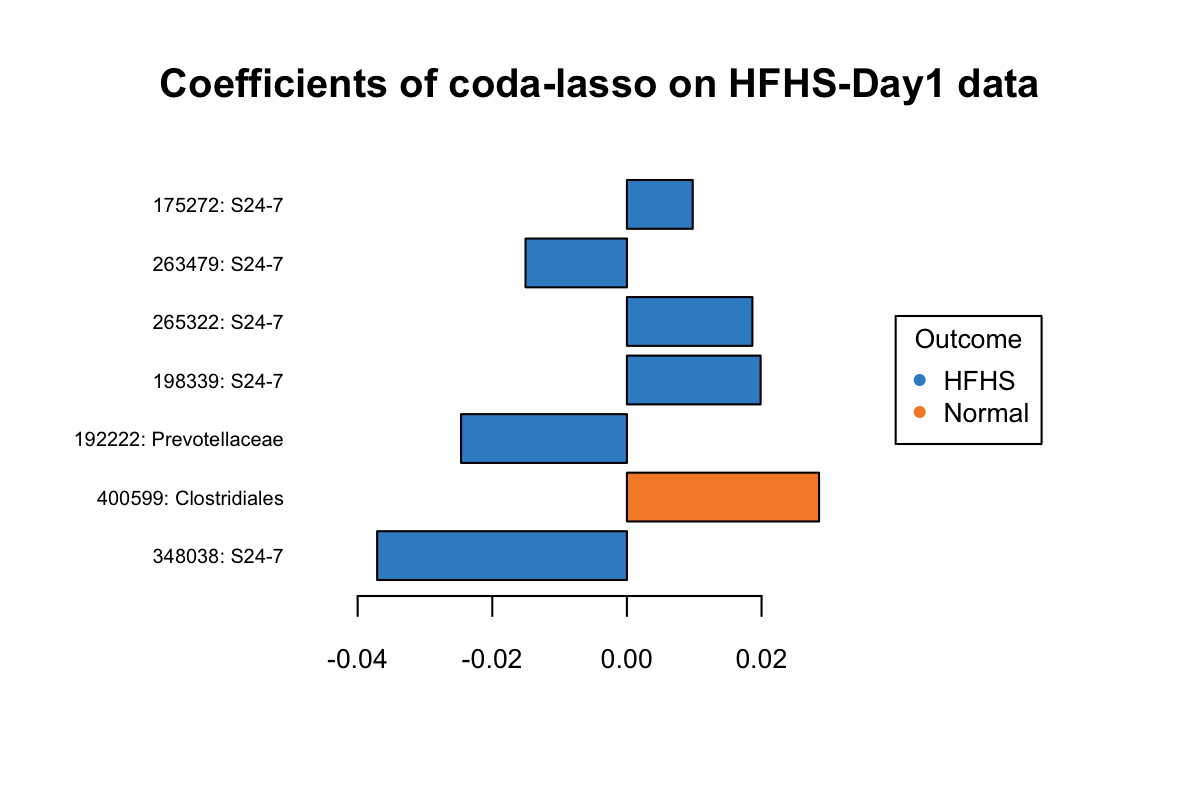
\includegraphics[width=1\linewidth]{./Generated_plots/loadcodaHFHS-1} 

}

\caption{The plotLoadings of selected variables with CoDA-lasso.}\label{fig:loadcodaHFHS}
\end{figure}

In Figure \ref{fig:loadcodaHFHS}, two OTUs \textbf{1105860: Allobaculum}
and \textbf{175272: S24-7} are more abundant in HFHS group but are
assigned with positive coefficients.

\begin{Shaded}
\begin{Highlighting}[]
\CommentTok{# CLR_lasso}
\NormalTok{HFHS.clr_coef <-}\StringTok{ }\NormalTok{HFHS.results_clrlasso}\OperatorTok{$}\NormalTok{coefficientsSelect}
\NormalTok{HFHS.clr_data <-}\StringTok{ }\NormalTok{HFHS.x[ ,HFHS.results_clrlasso}\OperatorTok{$}\NormalTok{varSelect]}
\NormalTok{HFHS.clr.plotloadings <-}\StringTok{ }\KeywordTok{plotcoefficients}\NormalTok{(}\DataTypeTok{coef =}\NormalTok{ HFHS.clr_coef, }
                                          \DataTypeTok{data =}\NormalTok{ HFHS.clr_data, }
                                          \DataTypeTok{Y =}\NormalTok{ HFHS.y, }
                                          \DataTypeTok{title =} \StringTok{'Coefficients of clr-lasso on HFHS-Day1 data'}\NormalTok{,}
                                          \DataTypeTok{OTU =}\NormalTok{ T,}
                                          \DataTypeTok{taxa =}\NormalTok{ HFHS.taxonomy)}
\end{Highlighting}
\end{Shaded}

\begin{figure}

{\centering 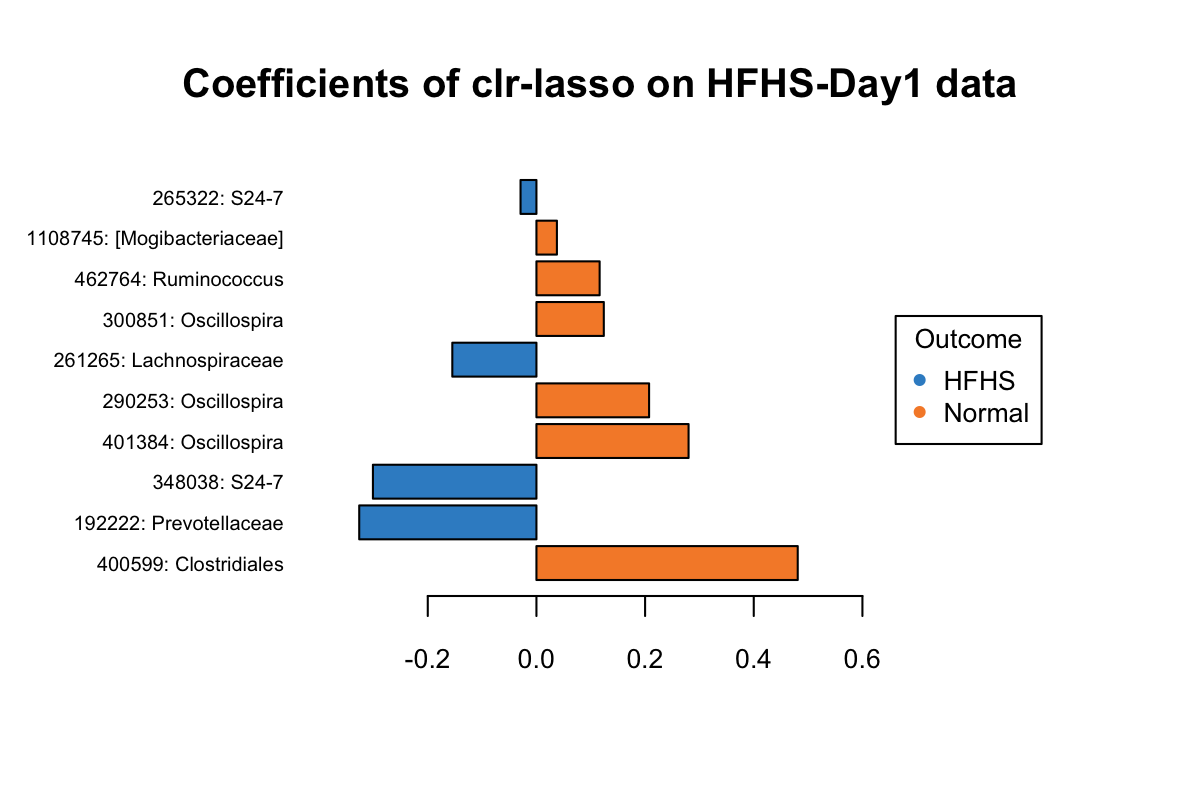
\includegraphics[width=1\linewidth]{./Generated_plots/loadclrHFHS-1} 

}

\caption{The plotLoadings of selected variables with CLR-lasso.}\label{fig:loadclrHFHS}
\end{figure}

\subsection{Trajectory plots}\label{trajectory-plots-1}

\begin{Shaded}
\begin{Highlighting}[]
\KeywordTok{TRAJ_plot}\NormalTok{(}\DataTypeTok{selectVar_coef_method1 =}\NormalTok{ HFHS.coda_coef, }\DataTypeTok{selectVar_coef_method2 =}\NormalTok{ HFHS.clr_coef, }
          \DataTypeTok{selectMethods =} \KeywordTok{c}\NormalTok{(}\StringTok{'CoDA-lasso'}\NormalTok{, }\StringTok{'CLR-lasso'}\NormalTok{), }\DataTypeTok{OTU =}\NormalTok{ T, }\DataTypeTok{taxa =}\NormalTok{ HFHS.taxonomy)}
\end{Highlighting}
\end{Shaded}

\begin{figure}

{\centering 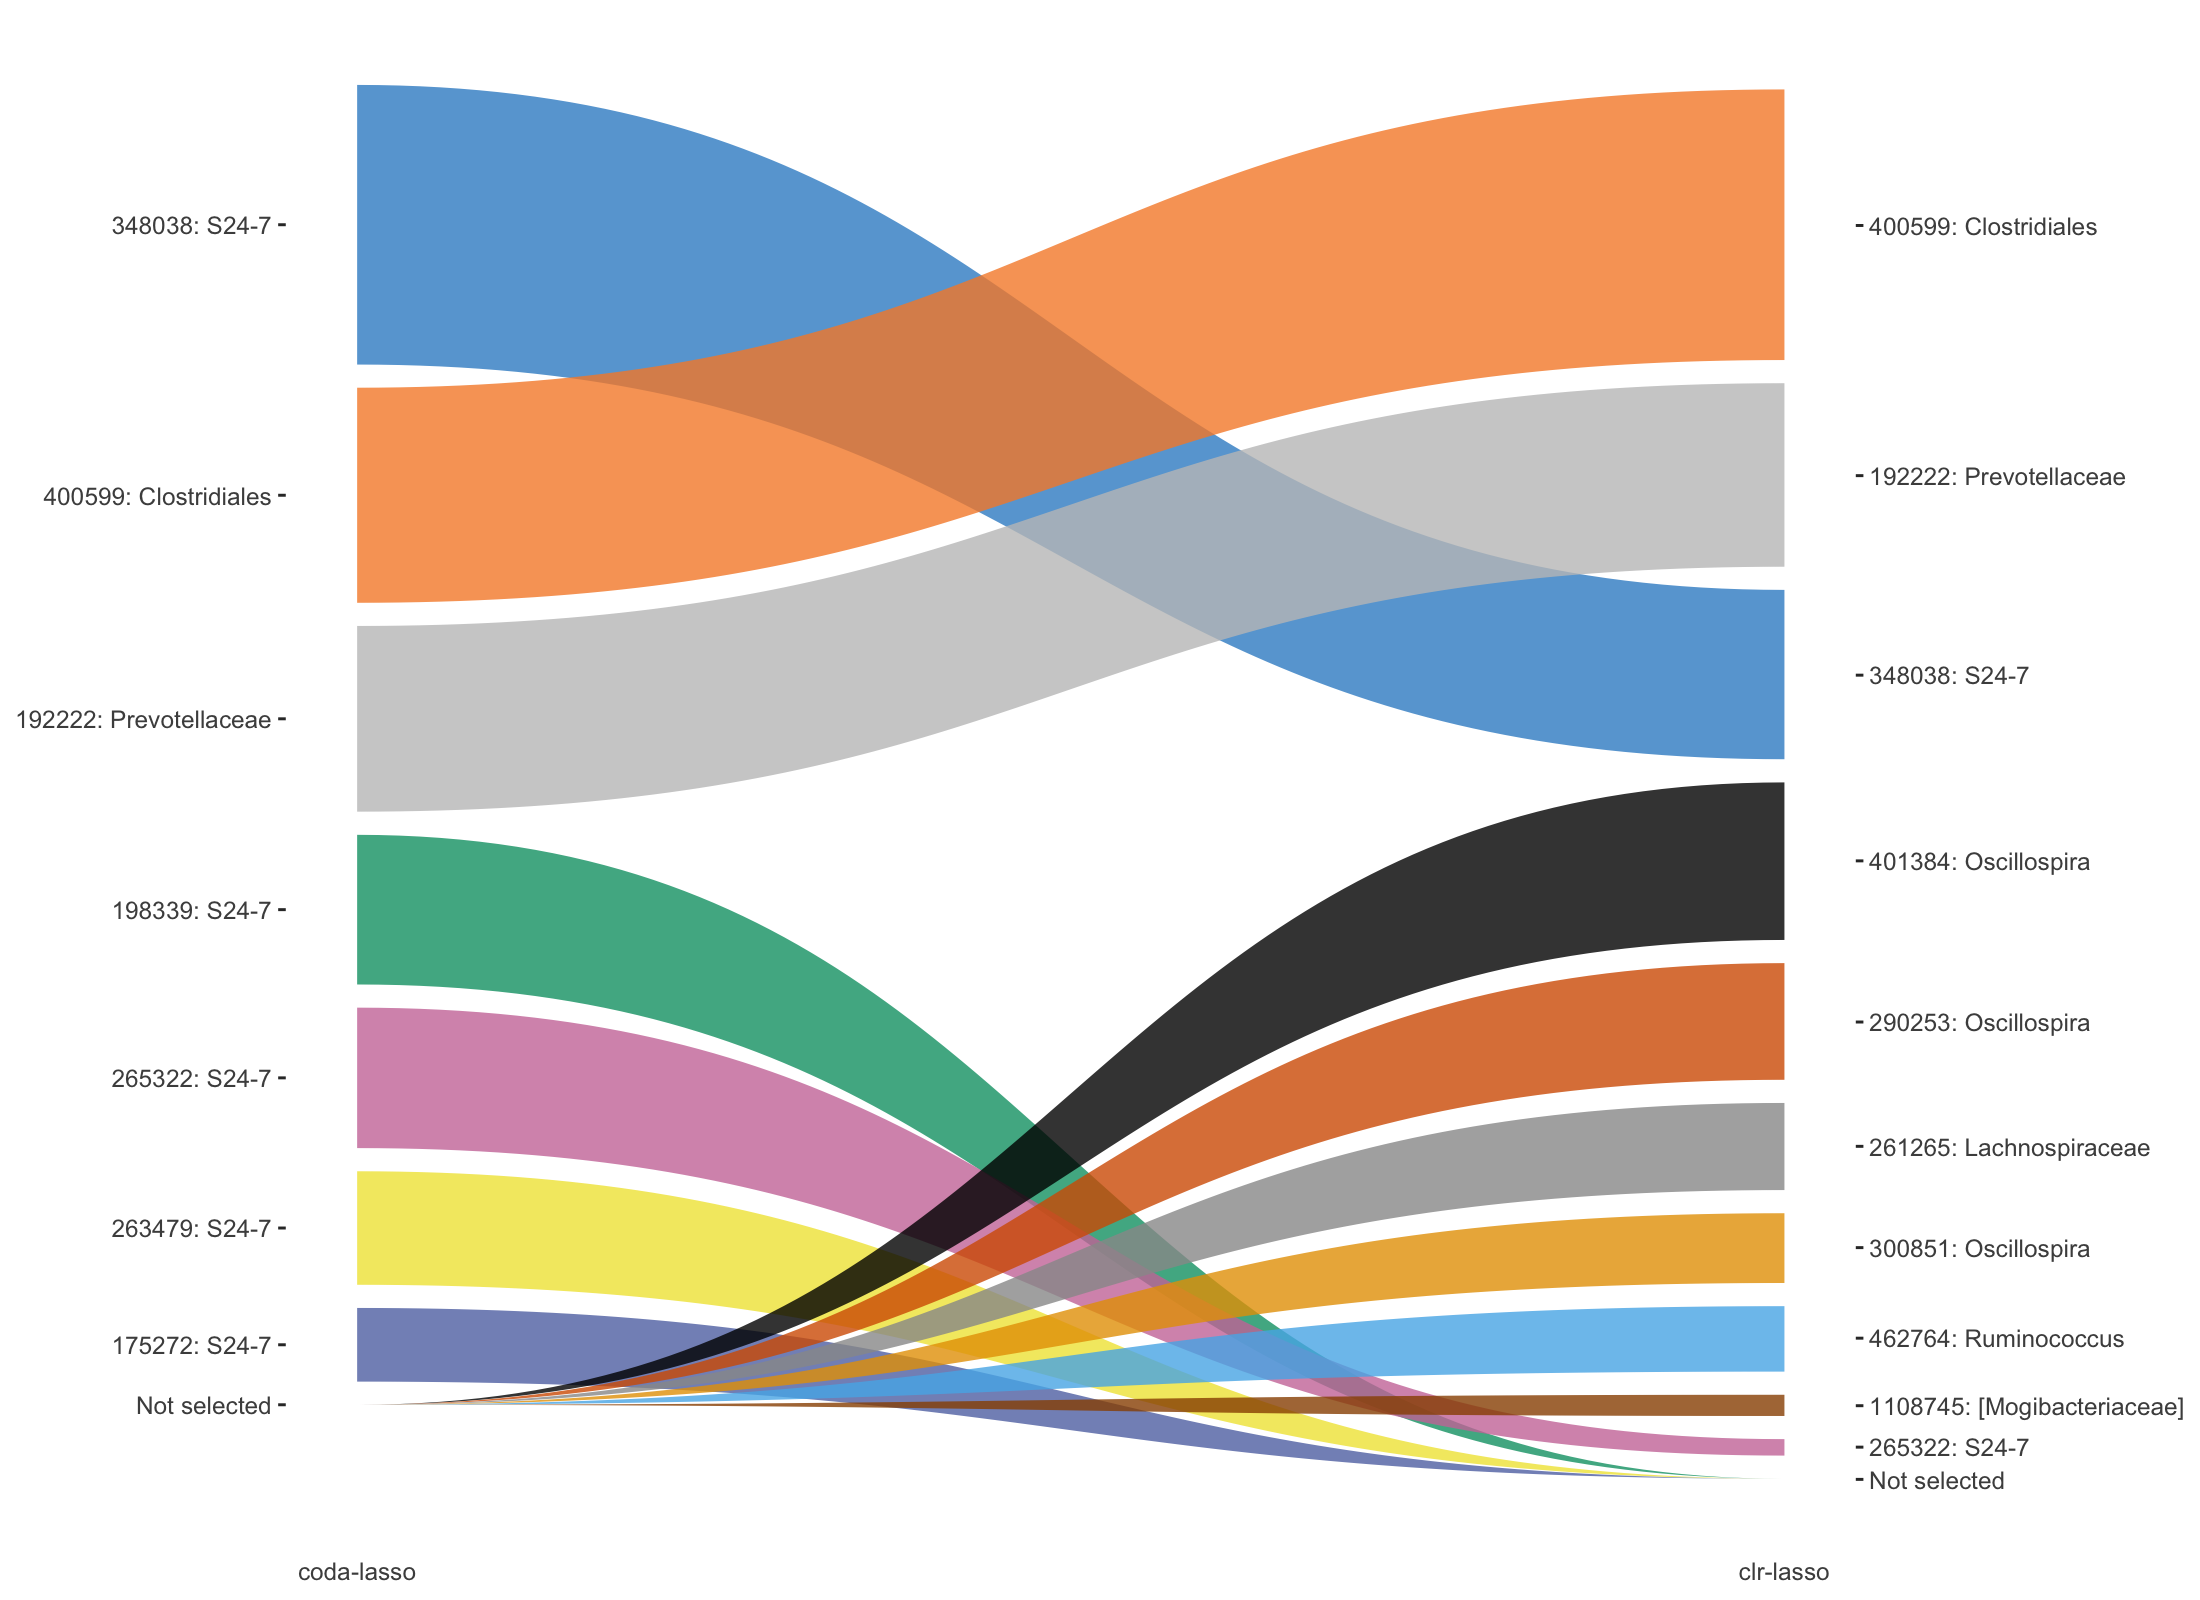
\includegraphics[width=1\linewidth]{./Generated_plots/trajHFHS-1} 

}

\caption{Trajectory plots of selected variables with both CoDA-lasso and CLR-lasso in HFHS-Day1 data.}\label{fig:trajHFHS}
\end{figure}

In Figure \ref{fig:trajHFHS}, top four OTUs selected with CLR-lasso are
also selected as top OTUs from CoDA-lasso but with different order. The
other OTUs are either selected by CoDA-lasso or CLR-lasso (except OTU
462764: Ruminococcus).

\subsection{GraPhlAn}\label{graphlan}

As we also have the taxonomic information of HFHS-Day1 data, we use
GraPhlAn to visualise the taxonomic information of the selected OTUs.
GraPhlAn is a software tool for producing high-quality circular
representations of taxonomic and phylogenetic trees
(\url{https://huttenhower.sph.harvard.edu/graphlan}). It is coded in
Python.

We first remove empty taxa (e.g.~species) and aggregate all these
selected variables into a list. Then we use function
\emph{graphlan\_annot\_generation()} to generate the input files that
graphlan python codes require. In the \textbf{save\_folder}, there are
two existing files: \textbf{annot\_0.txt} and \textbf{graphlan\_all.sh}.
After we generate our input files \textbf{taxa.txt} and
\textbf{annot\_all.txt}, we only need to run the
\textbf{graphlan\_all.sh} in the bash command line to generate the plot.

\begin{Shaded}
\begin{Highlighting}[]
\CommentTok{# remove empty columns}
\NormalTok{HFHS.tax_codalasso <-}\StringTok{ }\NormalTok{HFHS.tax_codalasso[,}\OperatorTok{-}\DecValTok{7}\NormalTok{] }
\NormalTok{HFHS.tax_clrlasso <-}\StringTok{ }\NormalTok{HFHS.tax_clrlasso[,}\OperatorTok{-}\DecValTok{7}\NormalTok{]}
\NormalTok{HFHS.tax_selbal <-}\StringTok{ }\NormalTok{HFHS.tax_selbal[,}\OperatorTok{-}\DecValTok{7}\NormalTok{]}

\NormalTok{HFHS.select.tax <-}\StringTok{ }\KeywordTok{list}\NormalTok{(}\DataTypeTok{CoDA_lasso =}\NormalTok{ HFHS.tax_codalasso, }
                        \DataTypeTok{CLR_lasso =}\NormalTok{ HFHS.tax_clrlasso, }
                        \DataTypeTok{selbal =}\NormalTok{ HFHS.tax_selbal)}

\KeywordTok{graphlan_annot_generation}\NormalTok{(}\DataTypeTok{taxa_list =}\NormalTok{ HFHS.select.tax, }
\DataTypeTok{save_folder =} \StringTok{'/Users/yiwenw5/Documents/GitHub/Methods_comparison/Methods_comparison/graphlan'}\NormalTok{)}
\end{Highlighting}
\end{Shaded}

\begin{figure}

{\centering 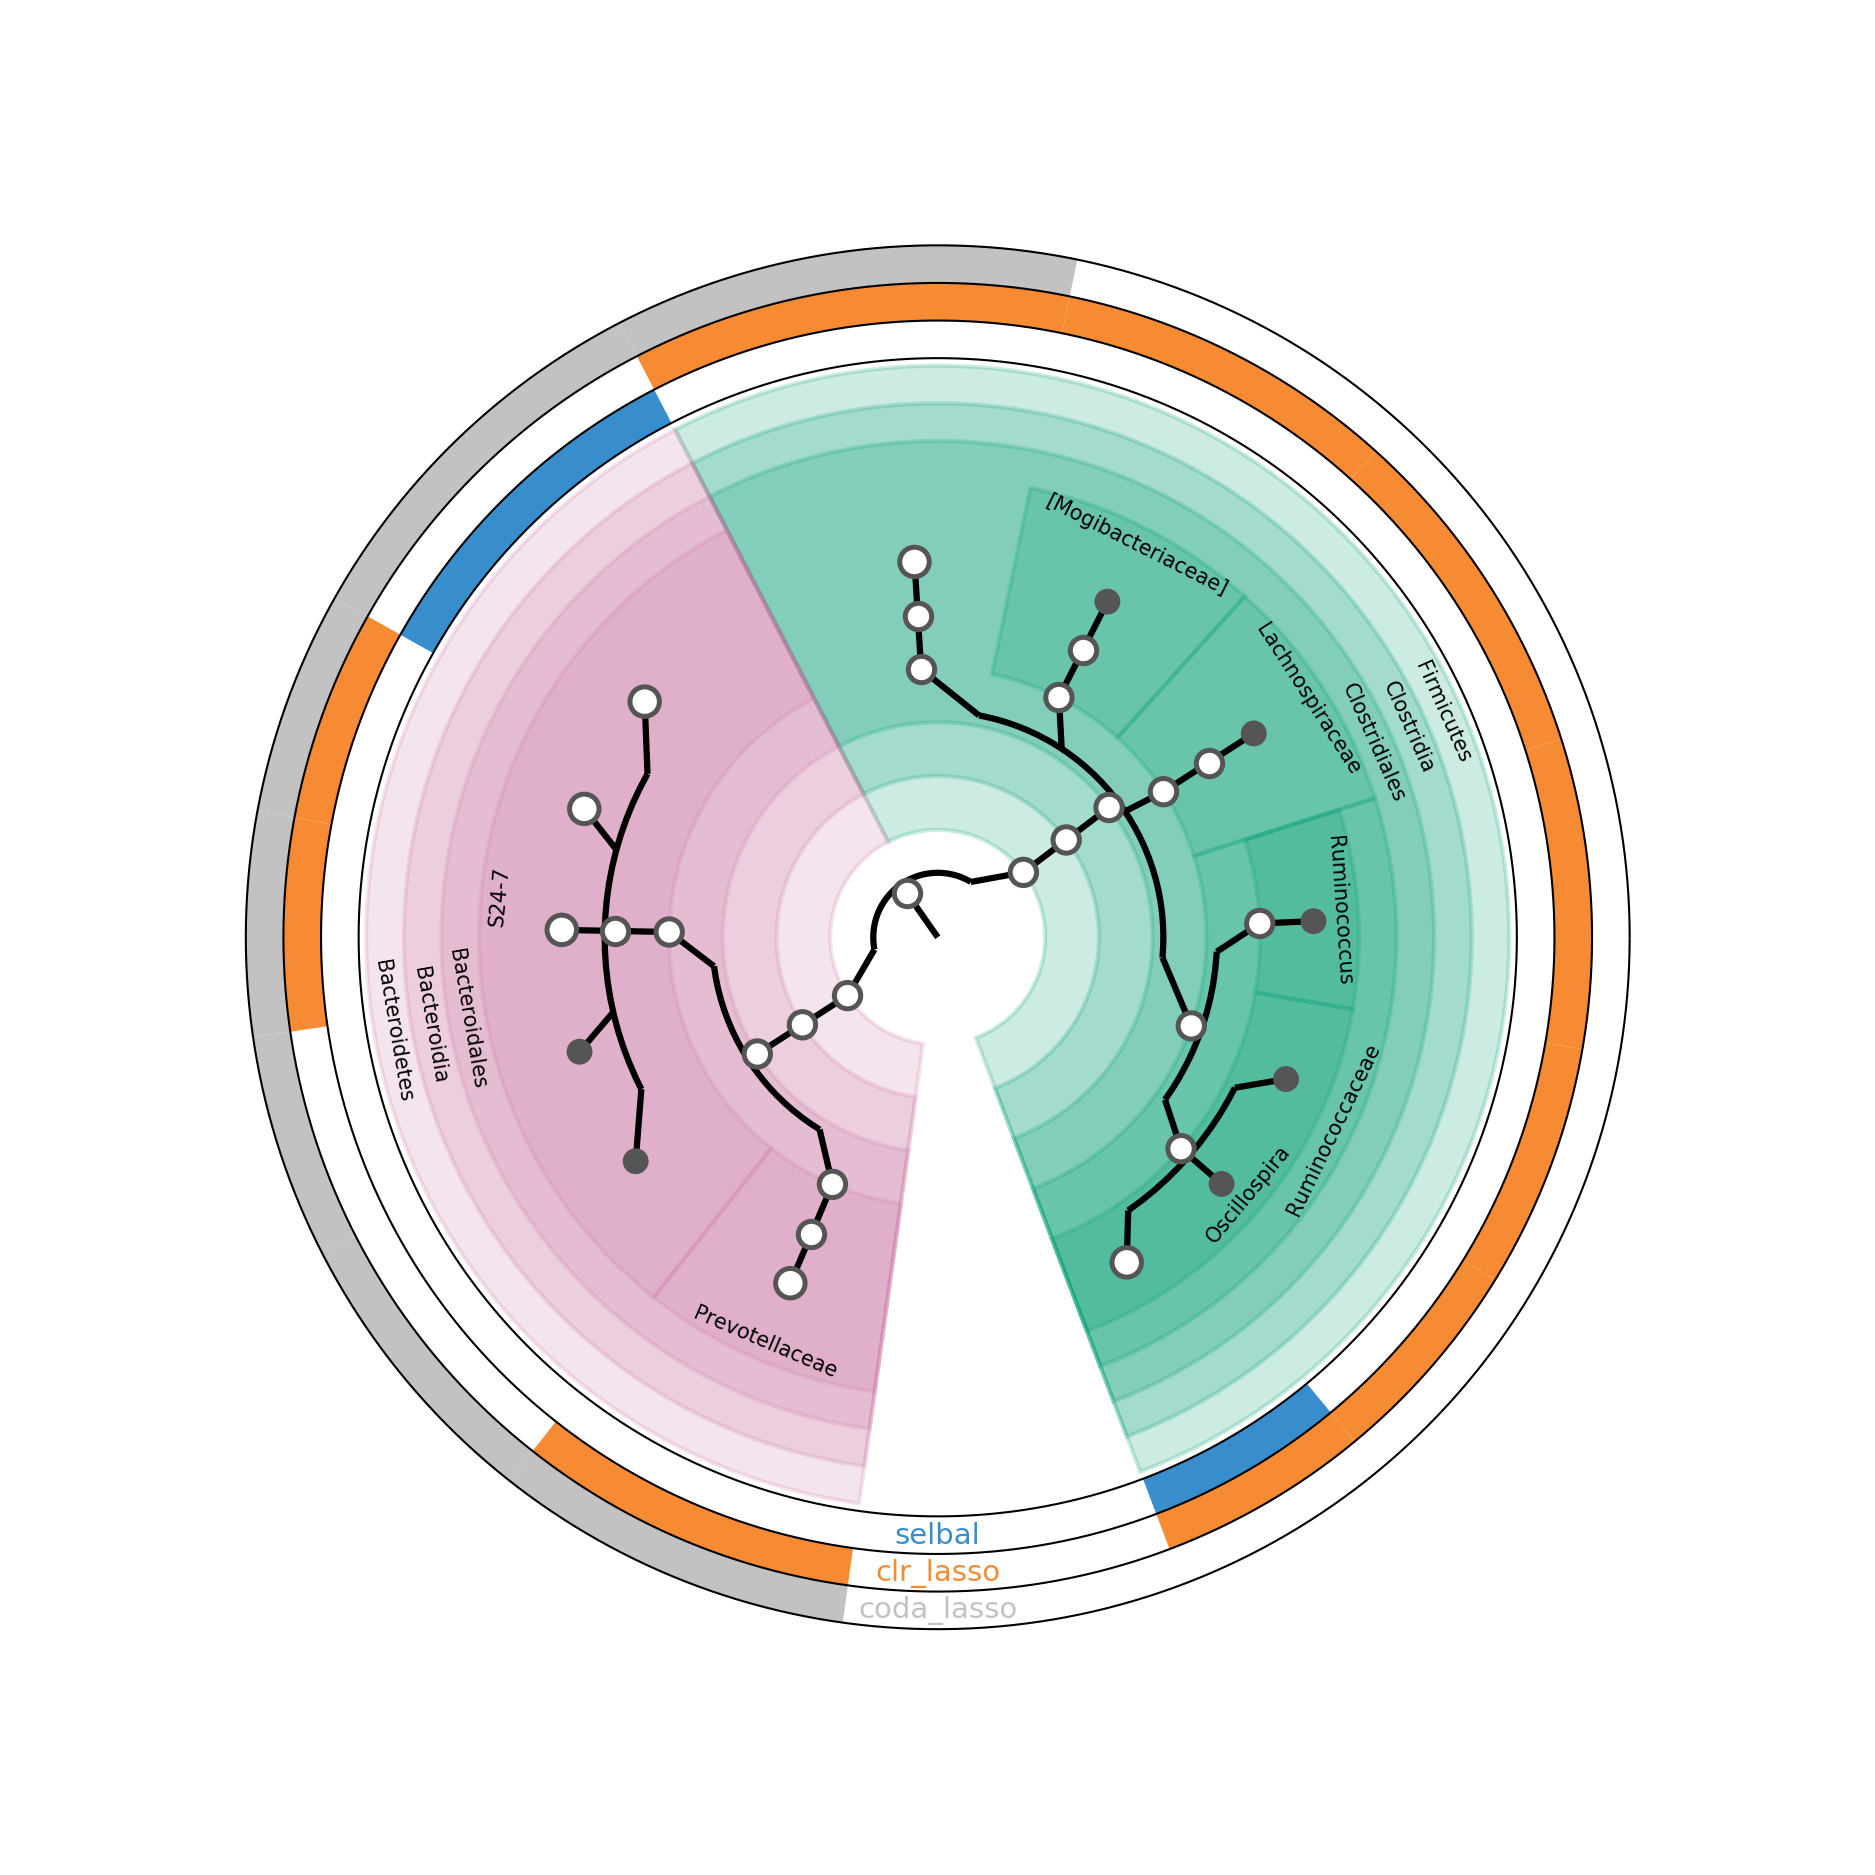
\includegraphics[width=1\linewidth]{./graphlan/taxa} 

}

\caption{GraPhlAn of selected taxa from different methods in HFHS-Day1 data.}\label{fig:graphlanHFHS}
\end{figure}

In Figure \ref{fig:graphlanHFHS}, the inner circle is a taxonomic tree
of selected OTUs. The outside circles indicate different selection
methods. If a proportion of a circle is coloured, it means that the
corresponding OTU is selected by the method labeled on the circle. If
the bottom nodes are coloured in gray, it indicates the OTUs are only
selected by one method.

\bibliography{book.bib}


\end{document}
